\documentclass[10pt,a4paper,footinclude=true,headinclude=true]{scrbook}

\newcommand{\myName}{Alessandro Candolini}
\newcommand{\myTitle}{Quantum Mechanics}
\newcommand{\mySubTitle}{}
\newcommand{\myLocation}{London}
\newcommand{\myTime}{\today}

% *****************************************************************************
%  Main packages
% *****************************************************************************

\usepackage[T1]{fontenc}
\usepackage[applemac]{inputenc}
\usepackage[english]{babel}
\usepackage[babel]{csquotes}
\usepackage{graphicx}
\usepackage[dvipsnames]{xcolor}


% typography
\usepackage[hyphenation]{impnattypo}
\usepackage[biblatex=true]{embrac}
\usepackage[final]{microtype}

\usepackage{listings}

\usepackage{makeidx}

\usepackage{tabularx}
\usepackage{booktabs}
\usepackage{subfig}
\usepackage{sidecap}
\usepackage{url}
\usepackage[font=small, noorphanfirst, indentfirst=false]{quoting}



% *****************************************************************************
% BIBLaTeX
% *****************************************************************************
\usepackage[%
style=philosophy-modern,
%style=philosophy-classic,
scauthorsbib,
hyperref,backref,
backend=biber,
square,
natbib,ibidtracker=false]{biblatex}

\bibliography{myBibliography9}

% ClassicThesis
\usepackage[pdfspacing,
  eulerchapternumbers,
  listings,
  eulermath,
  %style=arsclassica,
  parts,
  floatperchapter]{classicthesis}


% Footnote
\usepackage[perpage, symbol*, stable, multiple]{footmisc}
\setlength{\footnotemargin}{.6em}%

\usepackage{fnpct}
\setfnpct{add-punct-marks=:}
\setfnpct{add-punct-marks=;}

\usepackage{footnotebackref}
\makeatletter
\ifx\c@Hfootnote\undefined
\newcounter{Hfootnote}%
\fi

  \let\H@@footnotetext\@footnotetext
  \let\H@@footnotemark\@footnotemark
  \def\@xfootnotenext[#1]{%
    \begingroup
      \csname c@\@mpfn\endcsname #1\relax
      \unrestored@protected@xdef\@thefnmark{\thempfn}%
    \endgroup
    \ifx\@footnotetext\@mpfootnotetext
      \expandafter\H@@mpfootnotetext
    \else
      \expandafter\H@@footnotetext
    \fi
  }%
  \def\@xfootnotemark[#1]{%
    \begingroup
      \c@footnote #1\relax
      \unrestored@protected@xdef\@thefnmark{\thefootnote}%
    \endgroup
    \H@@footnotemark
  }%
  \let\H@@mpfootnotetext\@mpfootnotetext
  \long\def\@mpfootnotetext#1{%
    \H@@mpfootnotetext{%
      \ifHy@nesting
        \expandafter\hyper@@anchor\expandafter{%
          \Hy@footnote@currentHref
         }{#1}%
      \else
        \Hy@raisedlink{%
          \expandafter\hyper@@anchor\expandafter{%
            \Hy@footnote@currentHref
          }{\relax}%
        }#1%
      \fi
    }%
  }%
  \long\def\@footnotetext#1{%
    \H@@footnotetext{%
      \ifHy@nesting
        \expandafter\hyper@@anchor\expandafter{%
          \Hy@footnote@currentHref
        }{#1}%
      \else
        \Hy@raisedlink{%
          \expandafter\hyper@@anchor\expandafter{%
            \Hy@footnote@currentHref
          }{\relax}%
        }%
        \let\@currentHref\Hy@footnote@currentHref
        \let\@currentlabelname\@empty
        #1%
      \fi
    }%
  }%
  \def\@footnotemark{%
    \leavevmode
    \ifhmode\edef\@x@sf{\the\spacefactor}\nobreak\fi
    \stepcounter{Hfootnote}%
    \global\let\Hy@saved@currentHref\@currentHref
    \hyper@makecurrent{Hfootnote}%
    \global\let\Hy@footnote@currentHref\@currentHref
    \global\let\@currentHref\Hy@saved@currentHref
    \hyper@linkstart{link}{\Hy@footnote@currentHref}%
    \@makefnmark
    \hyper@linkend
    \ifhmode\spacefactor\@x@sf\fi
    \relax
  }%


\long\def\@footnotetext#1{%
      \H@@footnotetext{%
        \ifHy@nesting
         \hyper@@anchor{\@currentHref}{#1}%
       \else
         \Hy@raisedlink{\hyper@@anchor{\@currentHref}{\relax}}#1%
       \fi
     }}


  \def\@footnotemark{%
     \leavevmode
     \ifhmode\edef\@x@sf{\the\spacefactor}\nobreak\fi
     \H@refstepcounter{Hfootnote}%
     \hyper@makecurrent{Hfootnote}%
     \hyper@linkstart{link}{\@currentHref}%
     \@makefnmark
     \hyper@linkend
     \ifhmode\spacefactor\@x@sf\fi
     \relax
   }%

 \ifFN@multiplefootnote%
     \renewcommand*\@footnotemark{%
      \leavevmode
      \ifhmode
        \edef\@x@sf{\the\spacefactor}%
        \FN@mf@check
        \nobreak
      \fi
      \H@refstepcounter{Hfootnote}%
      \hyper@makecurrent{Hfootnote}%
      \hyper@linkstart{link}{\@currentHref}%
      \@makefnmark
      \hyper@linkend
      \FN@mf@prepare
      \ifhmode\spacefactor\@x@sf\fi
      \relax%
    }%
 \fi

\makeatother




\newenvironment{citazione}%
  {\begin{quotation}\small\ignorespaces}%
  {\end{quotation}}
\newenvironment{approfondimento}%
  {\begin{quotation}\small\ignorespaces}%
  {\end{quotation}}

\graphicspath{{./},{./Asymptote/}, {./Images/}}

% i.e.
\newcommand{\ie}{i.\,e.}
\newcommand{\Ie}{I.\,e.}
\newcommand{\eg}{e.\,g.}
\newcommand{\Eg}{E.\,g.}


% ********************************************************************
% hyperref
% ********************************************************************
\hypersetup{%
    colorlinks=true, linktocpage=true, pdfstartpage=1, pdfstartview=FitV,%
    breaklinks=true, pdfpagemode=UseNone, pageanchor=true, pdfpagemode=UseOutlines,%
    plainpages=false, bookmarksnumbered, bookmarksopen=true, bookmarksopenlevel=1,%
    hypertexnames=true, pdfhighlight=/O,%
    urlcolor=webbrown, linkcolor=RoyalBlue, citecolor=RoyalBlue,citecolor=webgreen,
    pdftitle={\myTitle},%
    pdfauthor={\textcopyright\ \myName},%
    pdfsubject={},%
    pdfkeywords={},%
    pdfcreator={pdfLaTeX},%
    pdfproducer={LaTeX con hyperref e ClassicThesis}%
}

\newcommand{\mail}[1]{\href{mailto:#1}{\texttt{#1}}}


% *****************************************************************************
% Math
% *****************************************************************************

% AMSmath packages
\usepackage{amssymb}

% comandi per gli insiemi numerici (serve il pacchetto amssymb)
\newcommand{\numberset}{\mathbb}
\newcommand{\N}{\numberset{N}}
\newcommand{\Z}{\numberset{Z}}
\newcommand{\Q}{\numberset{Q}}
\newcommand{\R}{\numberset{R}}
\newcommand{\C}{\numberset{C}}

\usepackage{braket}
\usepackage{cool}

% Theorems
\usepackage{amsthm}

\makeatletter
\newtheoremstyle{classicdef}%
{11pt}%                                   % Before
{11pt}%                                   % After
{}%                                       % Font
{}%                                       % Rientro (se vuoto, nessun rientro;
%                                         % \parindent = rientro dei capoversi)
{\scshape}%                               % Font
{:}%
{.5em}%
{}%
\makeatother

\theoremstyle{classicdef}
\newtheorem{theorem}{Theorem}[chapter]
\newtheorem{lemma}{Lemma}[chapter]
\newtheorem{definition}{Definition}[chapter]
\newtheorem*{homework}{Homework}
\newtheorem{exercise}{Exercise}[chapter]
\theoremstyle{remark}
\newtheorem*{remark}{Remark}
\renewcommand{\qedsymbol}{\rule{.5em}{.5em}}


\usepackage{caption}                      % Fancy captions and more.
\captionsetup{format=hang,font=small}
\captionsetup[table]{skip=\medskipamount}

\usepackage{mathtools}
\usepackage{flexisym}
\usepackage{breqn}
\DeclareFlexSymbol{\Gamma}  {Var}{latin}{00}
\DeclareFlexSymbol{\Delta}  {Var}{latin}{01}
\DeclareFlexSymbol{\Theta}  {Var}{latin}{02}
\DeclareFlexSymbol{\Lambda} {Var}{latin}{03}
\DeclareFlexSymbol{\Xi}     {Var}{latin}{04}
\DeclareFlexSymbol{\Pi}     {Var}{latin}{05}
\DeclareFlexSymbol{\Sigma}  {Var}{latin}{06}
\DeclareFlexSymbol{\Upsilon}{Var}{latin}{07}
\DeclareFlexSymbol{\Phi}    {Var}{latin}{08}
\DeclareFlexSymbol{\Psi}    {Var}{latin}{09}
\DeclareFlexSymbol{\Omega}  {Var}{latin}{0A}
\DeclareFlexSymbol{0}{Var}{latin}{30}
\DeclareFlexSymbol{1}{Var}{latin}{31}
\DeclareFlexSymbol{2}{Var}{latin}{32}
\DeclareFlexSymbol{3}{Var}{latin}{33}
\DeclareFlexSymbol{4}{Var}{latin}{34}
\DeclareFlexSymbol{5}{Var}{latin}{35}
\DeclareFlexSymbol{6}{Var}{latin}{36}
\DeclareFlexSymbol{7}{Var}{latin}{37}
\DeclareFlexSymbol{8}{Var}{latin}{38}
\DeclareFlexSymbol{9}{Var}{latin}{39}


\setkeys{breqn}{labelprefix={eq:}}


% Cleveref
\usepackage{cleveref}
\crefname{chapter}{\S}{\S}
\Crefname{chapter}{\S}{\S}



%%%% Other things

\newcommand*\openquote{\makebox(25,-12){\color{lightgray}\scalebox{5}{``}}}
\newcommand*\closequote{\makebox(25,-22){\color{lightgray}\scalebox{5}{''}}}

\usepackage{lettrine}
\usepackage{paralist}
\usepackage{enumitem}                          % Url.

% Costumizing  
\newcommand{\nto}[3]{#1 = #2, \ldots, #3}
\newcommand{\fullfunction}[3]{#1\colon#2\to#3}

% Intervals 
\usepackage{interval}
\newcommand{\commutator}[2]{\interval[scaled]{#1}{#2}}
\newcommand{\anticommutator}[2]{\interval[left closed fence={\{}, right closed fence={\}}, scaled]{#1}{#2}}



\usepackage{cancel}


\NewDocumentCommand\K{}{\ensuremath{\mathbb{K}}}
\DeclareDocumentCommand\ii{}{\ensuremath{\__skmath_imaginary_unit:n{i}}}
\DeclareDocumentCommand\jj{}{\ensuremath{\__skmath_imaginary_unit:n{j}}}
% Cando's addition: k for quaternions
\DeclareDocumentCommand\kk{}{\ensuremath{\__skmath_imaginary_unit:n{k}}}
\DeclareDocumentCommand\ee{}{\ensuremath{\__skmath_imaginary_unit:n{e}}}

% Cando's addition: L spaces (add stared version without left /right
  \NewDocumentCommand\LspaceSet{}{\ensuremath{\mathrm{L}}}
  \NewDocumentCommand\lspaceSet{}{\ensuremath{l}}
\DeclareDocumentCommand\lspace{m}{%
	 \ensuremath{\lspaceSet^{#1}}
}

\DeclareDocumentCommand\Lspace{sd<>om}{%
  \IfBooleanTF{#1}{
      \IfNoValueTF{#2}
      {
	 \IfNoValueTF{#3}
	 {\ensuremath{\LspaceSet^{#4}}}
	 {\ensuremath{\LspaceSet^{#4}\left( #3\right)  }}
      }{
	 \IfNoValueTF{#3}
	 {\ensuremath{#2}^{#4}}
	 {\ensuremath{#2^{#4}\left( #3\right)  }}
      }
   }
   {
      \IfNoValueTF{#2}
      {
	 \IfNoValueTF{#3}
	 {\ensuremath{\LspaceSet^{#4}}}
	 {\ensuremath{\LspaceSet^{#4}( #3)  }}
      }{
	 \IfNoValueTF{#3}
	 {\ensuremath{#2}^{#4}}
	 {\ensuremath{#2^{#4}( #3)  }}
      }
   }
}



% Cando's addition: Norm with optional macro argument
\DeclareDocumentCommand\norm{som}{%
  \IfBooleanTF{#1}{
     \IfNoValueTF{#2} {
     	 \ensuremath{\Vert#3\Vert}
     }{
      	\ensuremath{\Vert#3\Vert\c_math_subscript_token{#2}}%
     }
  }{
     \IfNoValueTF{#2} {
     	 \ensuremath{\left\Vert#3\right\Vert}
     }{
      	\ensuremath{\left\Vert#3\right\Vert\c_math_subscript_token{#2}}%
     }
  }
}
% Cando's addition: Norm with optional macro argument
\DeclareDocumentCommand\abs{som}{%
  \IfBooleanTF{#1}{
     \IfNoValueTF{#2} {
     	 \ensuremath{\vert#3\vert}
     }{
      	\ensuremath{\vert#3\vert\c_math_subscript_token{#2}}%
     }
  }{
     \IfNoValueTF{#2} {
     	 \ensuremath{\left\vert#3\right\vert}
     }{
      	\ensuremath{\left\vert#3\right\vert\c_math_subscript_token{#2}}%
     }
  }
}

% Cando's addition: complex conjugation
\DeclareDocumentCommand\conj{sm}{%
   \IfBooleanTF{#1}{
      \ensuremath{\left(#2\right)^{*}}%
  }{
      \ensuremath{#2^{*}}%
  }
}

% Cando's addition: Adjoint
\DeclareDocumentCommand\adj{sm}{%
   \IfBooleanTF{#1}{
      \ensuremath{\left(#2\right)^{\dagger}}%
  }{
      \ensuremath{#2^{\dagger}}%
  }
}






% *****************************************************************************
% Main
% *****************************************************************************
\begin{document}
\pagenumbering{roman}
\pagestyle{plain}
%*******************************************************
% Titlepage
%*******************************************************
\newcommand{\suftitolo}[2]{\textcolor{Maroon}{#1}\textcolor{Black!30}{#2}}
\begin{titlepage}
	% if you want the titlepage to be centered, uncomment and fine-tune the line below (KOMA classes environment)
%	\begin{addmargin}[-1cm]{-3cm}
	\parindent0pt
		\begin{picture}(0,0)
		\fontsize{60}{60}\selectfont
		   \setlength{\unitlength}{1mm}
		      \put(124,-200){%
		%\rotatebox{0}{\suftitolo{Q}{uantum} 
		%	\suftitolo{M}{echanics}}}%
	     }
		\end{picture}
	
	\null\vspace{\stretch{1}}
	
	\large \myName
		\vskip4ex
			\hrule
		\vskip4ex
	{\bfseries\Huge\color{Maroon} 
	   {\fontsize{40}{40}\selectfont
		   \suftitolo{Q}{uantum} 
			\suftitolo{M}{echanics}
		     }
	   %\myTitle\\[1ex]
	   }%
	   {\large \mySubTitle} 
	
	\vspace{\stretch{4}}
	
	\myTime
  %\end{addmargin}       
\end{titlepage}



%\begin{titlepage}
%{
%        \large  
%
%        \hfill
%
%        \vfill
%
%        \begingroup
%            \color{Maroon}\spacedallcaps{\myTitle} \\ \bigskip
%        \endgroup

%        \spacedlowsmallcaps{\myName}

%        \vfill

        %\includegraphics[width=6cm]{gfx/TFZsuperellipse_bw} \\ \medskip

        %\mySubtitle \\ \medskip   
        %\myDegree \\
        %\myDepartment \\                            
        %\myFaculty \\
        %\myUni \\ \bigskip

%\vfill
%}

%        \textsw{\myTime}
%\ -- \myVersion

%        \vfill                      

%    \end{center}  
 % \end{addmargin}       
%\end{titlepage}   





%*******************************************************
% Titlepage
%*******************************************************
%\begin{titlepage}
%\pdfbookmark{Titlepage}{Titlepage}
%\changetext{}{}{}{((\paperwidth  - \textwidth) / 2) - \oddsidemargin - \hoffset - 1in}{}
%\null\vfill
%\begin{center}
%\large
%\sffamily

%\bigskip

%{\Large\spacedlowsmallcaps{\myName}} \\

%\bigskip

%{\huge\spacedlowsmallcaps{\myTitle} \\
%}

%\bigskip
%{\large\spacedlowsmallcaps{\mySubTitle}} \\

    
%\vfill
%\vfill
%\vfill
%					{\normalsize
					
%        \myTime}
%\end{center}
%\end{titlepage}



\clearpage



%*******************************************************
% Titleback
%*******************************************************
%\thispagestyle{empty}
%	\null
%	  \vfill
%	       \ifx\myName\@empty\else
%	          \noindent Copyright \copyright{} \the\year~\myName\\[1ex]
 %                 All rights reserved.
%	      \fi
%	\vfill	
%    %\section*{Colophon}
%	{\small \noindent Typeset by \myName{} using \LaTeX2e.} \\
%\hrule
%\bigskip

%{\small \noindent{\spacedlowsmallcaps{E-mail}}: 
%\mail{alessandro.candolini@gmail.com}}

%% copyrightpage
\thispagestyle{empty}
\begingroup
%\footnotesize
\small
\parindent 0pt
\parskip \baselineskip
	\null
  \vfill
\ifx\myName\@empty\else
\noindent
Copyright \textcopyright{} \the\year~\myName\\
All rights reserved.

	  \vfill

%\begin{center}
% 12 11 10 09 08 07\hspace{2em}8 7 6 5 4 3 %2 
%\end{center}

%\begin{center}
%\begin{tabular}{ll}
%First edition:  & July 2012 \\
%\end{tabular}
%\end{center}

\vfill

%\myName\\
%\hspace*{2em} \myTitle / \myName{}. -- \\
%\hspace*{1em} 1st Herries Press ed. \\
%\hspace*{2em} p. \hspace*{2em} cm. \\
%\hspace*{2em} Includes illustrations, bibliographical references and index. \\
%\hspace*{2em} ISBN \\
%\hspace*{2em} 1. Book design \hspace*{2em} I. Title


\vfill

%Typeset by \myName{} using \LaTeX2e. \\
%\hrule
%\bigskip
%\spacedlowsmallcaps{E-mail}: \mail{alessandro.candolini@gmail.com}
%The Herries Press, \\
%Normandy Park, WA \\
%\texttt{herries dot press (at) earthlink dot net}

%%%%{\LARGE\plogo}
\vspace*{2\baselineskip}


\endgroup
\clearpage




%\thispagestyle{empty}

%\hfill

%\vfill

%\noindent\myName: \textit{\myTitle}
%\textcopyright\ \MakeTextLowercase{\myTime}.

%\medskip
%\medskip
%\noindent{\spacedlowsmallcaps{E-mail}}: \\
%\mail{alessandro.candolini@gmail.com}

%\vspace{1cm}
%%\hrule
%\bigskip

%%\noindent The titlepage reproduces an engraving of Maurits Cornelis Escher, titled \emph{Plane Filling with Birds} (the picture is obtained from \url{http://www.mcescher.com/}).



%*******************************************************
% Dedication
%*******************************************************
\cleardoublepage
\thispagestyle{empty}
%\phantomsection 
\pdfbookmark[1]{Dedication}{Dedication}

\vspace*{3cm}

\begin{quotation}

   \openquote In the good old days, theorizing was like sailing between islands of
   experimental evidence. And, if the trip was not in the vicinity of the
   shoreline (which was strongly recommended for safety reasons) sailors where
   continuously looking forward, hoping to see land --- the sooner the better.
   
   Nowadays, some theoretical physicists (let us call them sailors) [have]
   found a way to survive and navigate in the open sea of pure theoretical
   constructions. Instead of the horizon, they look at stars, which tell them
   exactly where they are. Sailors are aware of the fact that the stars will
   never tell them where the new land is, but they may tell them their position
   on the globe. 

   Theoreticians become sailors simply bacause they just like it. Young people,
   seduced by capitans forming crews to go to a Nuevo El Dorando \omissis{} soon
   realize that they will spend all their life at sea. Those who do not like
   sailing desert the voyage, but for the true potential sailors the sea become
   their passion. They will probably tell the alluring and frightening truth to
   their students --- and the proper people will join their ranks.~\closequote

   \begin{flushright}
      ---  Andrei Losev
   \end{flushright}

\end{quotation}

\medskip

%\begin{center}
%    Dedicated to the loving memory of Rudolf Miede. \\ \smallskip
%    1939\,--\,2005
%\end{center}











\pagestyle{scrheadings}
%*******************************************************
% Contents
%*******************************************************
\cleardoublepage
%\phantomsection
%\pdfbookmark{\contentsname}{tableofcontents}
\setcounter{tocdepth}{2}

\begingroup 
    \let\clearpage\relax
    \let\cleardoublepage\relax
    \let\cleardoublepage\relax
%\dominitoc
\tableofcontents
\endgroup
\markboth{\spacedlowsmallcaps{\contentsname}}{\spacedlowsmallcaps{\contentsname}} 

\cleardoublepage


\chapter*{Preface}
\markboth{\spacedlowsmallcaps{Preface}}{\spacedlowsmallcaps{Preface}}
\addcontentsline{toc}{chapter}{\tocEntry{Preface}}

\smallskip

\noindent\textsw{\myLocation, \myTime}


\begin{flushright}
        \myName
\end{flushright}


\cleardoublepage
\cleardoublepage
\cleardoublepage
\mainmatter
\cleardoublepage
\pagenumbering{arabic}
\part{The basis}

% !TEX encoding = latin1
% !TEX TS-program = pdflatex
% !TEX root = ../handout_qft.tex
% !TEX spellcheck = it-IT

%*******************************************************
% Chapter 1
%*******************************************************

\myChapter{Schwinger's own way to teach quantum mechanics}
%\myChapter{Schwinger's approach to quantum mechanics}
\label{chp:fundamentals} 

%\minitoc\mtcskip

\begin{refsection}
\begin{quoting}
   \openquote 
   I presume that all of you have already been exposed to some undergraduate
   course in Quantum Mechanics, one that leans heavily on de Broglie waves and
   the Schroedinger equation. I have never thought that this simple wave
   approach was acceptable as a general basis for the whole subject, and I
   intend to move immediately to replace it in your mind by a foundation that
   \emph{is} perfectly general.~\closequote
   \begin{flushright}
       J. Schwinger,
       \emph{Quantum Mechanics. Symbolism of Atomic Measurements}
       \textcite{Schwinger:2001}.
    \end{flushright}
\end{quoting}

\section{Introduction}

\lettrine{C}{ompared} 
with other traditional areas of physics, quantum mechanics is not easy. 
It often lacks physical intuitition and it relies on heavy mathematical
background from the very beginning.
As we shall see shortly, 
topics like Heisenberg's uncertanty principle, the intriguing role of probability in predicting the
outcomes of a quantum measurement, entanglement and superposition of quantum
states, etc
asks immediately for a theoretical framework capable of supporting and
describing such behaviors. The phase space in Hamiltonian classical dynamics 
simply not suitable because it is  not
able to include such phenomena, 
are built  in the formalism 
(at least in its traditional construction)
does not offer the tools. 
it is not enugh flexible. 
Naturally leading from the very beginning to adopt .


For example, incompatibility between physical measurable quantities like position and
momentum, which is at the root of uncetainty principle, can be described in
terms of \emph{non-commutative} objects, leading naturally to adopt matrices or
operators (instead of usual numbers) to describe position and momentum.
As we shall see, the canonical commutation relations imposed event further
requirements: they can't be realized in finite-dimensional vector spaces,
so we need to look at infinite-dimensional (Hilbert) spaces. 

Can we avoid Hilbert space?
As we shall see in the last part, other descriptions are possible, in
particular the path integral approach to quantum mechanics due to Feynman. 

In chapter~3, we will present and throughly discuss  all the postulates of  
non-relativistic quantum
mechanics. 
They have been distillized in the Twenties and Thirtees of '900 after  at least two
decades of strong and fashinating efforts, 
theoretical and experimental progress, wrong
attempts, mistakes, etc 
made by the intellectual fathers of quantum mechanics 
to eventually capture the essential  rules underlying 
the microscopic behavior of particles.

For example, consider classical electrodynamics. 
One can ask: are fields ``necessary''?


% Navigando a vista in un mare allora sconosciuto, inciampando negli
% imprevisti, 
% un percorso di intuizioni poi dimostratesi erronee, tentativi andati a vuoto
% vicoli ciechi, intuizioni che hanno spronato direzioni importanti per poi non
% trovare posto nella costruzione definitiva. 
% Questo lavoro e' confluito e si riassume nei postulati della meccanica
% quantistica.
% La loro validita' si poggia in ultima analisi sull'accordo con i fatti  sperimentali ovviamente, come per ogni
% branca della fisica. La loro forma e' quella a cui sono approdotati coloro
% che 
% Tuttavia, l'elevato livello di astrazione che li caratterizza, puo' 



\begin{figure}
   \centering
   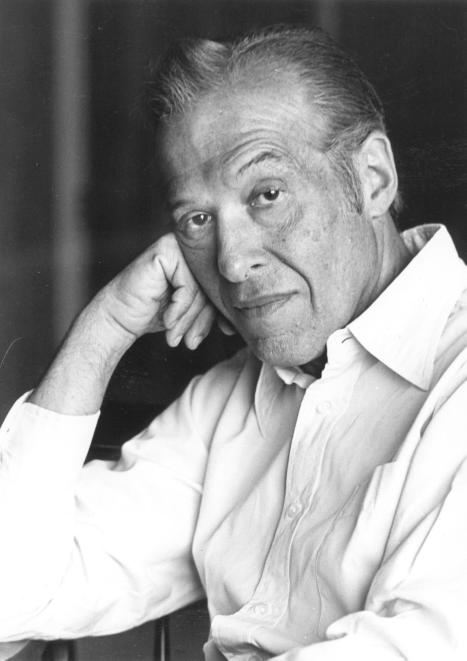
\includegraphics[scale=.35]{./Images/schwinger}
   \caption{Julian Seymour Schwinger (February 12, 1918 -- July 16, 1994) }
\end{figure}

\printbibliography[heading=subbibliography]
\end{refsection}


%*******************************************************
% Chapter 2
%*******************************************************



\myChapter{Linear operators in Hilbert spaces}

\begin{refsection}


%\lettrine{T}{he} 
The operator formulation of standard non-relativistic quantum mechanics is based on the spectral theory of linear self-ajoint operators (bound or unbound) in complex separable Hilbert spaces.
This chapter provides the necessary mathematical groundwork in functional analysis to approach non-relativistic quantum mechanics in full generality. 
Readers already acquainted with these concepts may choose to jump to the next chapter to see how the mathematical theory is applied in quantum mechanics. 
  Familiarity with basic linear algebra (eg, at the level of) and real analysis (\eg, at the level of) is assumed. 

% In formulating quantum mechanics, physicists often rely on Dirac's notation, a potent mnemonic technique that, at first glance, lacks strict mathematical rigor. Nonetheless, it is feasible to create a correspondence between Dirac's notation and the rigorous theorems of functional analysis, as we will delve into in subsequent sections.

This chapter is based on \textcite{Reed.Simon:1980}. 
Some other books that have been helpful while writing this chapter includes:
\textcite{Teschl:2009,Berberian:1976,Hutson.Pym:1980,Debnath.Mikusinski:2005,Helmberg:1969}.


  \section{Metric spaces}

Metric spaces are sets endowed with an additional algebraic structure that attaches significance to the concept of ``distance'' between each pair of elements in the set.
Metric spaces provide a natural context in which to develop concepts like continuity, convergence, and more.

  \begin{definition}[distance]
    Let $A$ be a set. 
    A ``distance'' (or ``metrics'') over $A$ is
   any application $\fullfunction{d}{A\times
      A}{\interval[open right]{0}{+\infty}}$, satisfying the following requirements: 
   \begin{enumerate} [label=(\alph*)]
      \item 
	 \label{item:distance1}
	 \begin{math}
	    d(\varphi,\psi) \geq 0 \condition{$\forall (\varphi,\psi)\in A
	       \times A$}
	 \end{math}
	 (nonnegativity);
      \item 
	 \label{item:distance2}
       $d(\varphi,\psi) = 0$ \emph{if and only if} $\varphi = \psi$
	 (\ie, for every $\psi \in A$, the distance from itself is always zero and $\psi$ is also the only element in $A$ at zero distance from
	 $\psi$);
      \item 
	 \label{item:distance3}
	 \begin{math}
	    d(\varphi,\psi) = d(\psi,\varphi) \condition{$\forall
	       (\varphi,\psi)\in A 
	       \times A$}
	 \end{math}
	 (\ie, the distance is a symmetric function of its arguments);
      \item 
	 \label{item:distance4}
	 \begin{math}
	    d(\varphi,\psi) \leq  d(\psi,\eta) + d(\eta,
	    \psi)\condition{$\forall (\varphi,\psi,\eta)\in A
	       \times A\times A $}
	 \end{math} (the so-called ``triangle inequality'').
   \end{enumerate}
  \end{definition}

  \begin{definition}[metric space]
    A ``metric space'' is an ordered pair $(A, d)$, where $A$is a set and $\fullfunction{d}{A\times A}{A}$ is a distance on $A$.
  \end{definition}


  Given a metric space $(A,d)$, the elements of $A$ are often referred to as ``points'' in this context. 

  The next sections will provide examples of metrics spaces where the distance arises from other algebraic structures (\ie, norms and inner products). Without pretending to extensively develop the theory of metrics spaces in this section, it's worth briefly summarising elements of topology of metric spaces. In particular, the notions of continuity, convergence, etc can be formulated quite generally in the context of metrics spaces.

  \begin{definition}[continuity]
    Let $(A,d)$ and $(A', d')$ be metric spaces and $\fullfunction{f}{A}{A'}$ a function.
    $f$ is ``continuous'' at a point $\varphi\in A$  (with respect to the given metrics) if for any positive real number $\varepsilon > 0$, there exists a positive real number $\delta > 0 $ such that for every $\psi \in A$, $d(\varphi, \psi) < \delta$ implies $d'(f(\varphi), f(\psi) ) < \varepsilon$. Formally, 
    \begin{dmath}[label={eq:continuity}]
      (\forall \varepsilon > 0)
      (\exists \delta > 0 )
      (\forall \psi \in A) 
      \left(d(\varphi, \psi) < \delta \Rightarrow d'(f(\varphi), f(\psi)) < \varepsilon \right)
    \end{dmath}.
  \end{definition}
  The notion can be further generalised to functions between \emph{topological spaces} in which there is generally no formal notion of distance.
   

  \section{Topology of metrics spaces}

  \subsection{Completeness}

  \subsection{Compactness} 


\section{Banach and Hilber spaces}

Unless stated otherwise, let $\K $ denote either the field of real numbers
$\R$ or the field of complex numbers $\C$.
(It is possible to develop the theory also for the skew-field of quaternions,
but this case will not be taken  into account  here in order to avoid dealing with the
non-commutativity of the quaternionic product.)


\begin{definition}[norm]
   Let 
   $X$ be any vector space over $\K$.
   A ``norm'' on $X$ is any application  $X \to \R$  hereafter denoted by $\norm{\cdot}$ 
   satisfying the following properties:
   \begin{enumerate} [label=(\alph*)]
	 %[(a)]
      \item 
	 \label{item:norm1}
	 \begin{math}
	    \norm{\varphi} \geq 0  \condition{$\forall \varphi \in X$}
	 \end{math}
	 (nonnegativity);
      \item 
	 \label{item:norm2}
	 $\norm{\varphi} = 0$ if and only if $\varphi = 0$
	 (faithfulness)
      \item 
	 \label{item:norm3}
	 \begin{math}
	 \norm{\lambda \varphi} = \abs{\lambda} \norm{\varphi}
	 \condition{$\forall\lambda\in \K$ and $\forall\varphi \in X$}
      \end{math}
	 (positive homogeneity);
      \item 
	 \label{item:norm4}
	 \begin{math}
	 \norm{\varphi + \psi} \leq \norm{
	    \varphi} + \norm{\psi}
	 \condition*{\forall (\varphi,\psi) \in X \times X} 
      \end{math}
      (subadditivity).
   \end{enumerate}
\end{definition}

A norm on $X$ can be viewed as a way to define a ``length'' of the vectors belonging
to $X$.

\begin{remark}
   \Cref{item:norm1} is redundant: 
   it follows from
   \cref{item:norm2,item:norm3,item:norm4}.
   For every $\varphi\in X$, \cref{item:norm3} implies $\norm{-\varphi} = \norm{\varphi}$, 
   from \cref{item:norm4} it follows that $\norm{\varphi + (- \varphi)} \leq 
   \norm{\varphi} + \norm{\varphi}$, and 
   \cref{item:norm2} implies $\norm{\varphi-\varphi} = 0$, so $\norm{\varphi}
   \geq 0$.
\end{remark}

\begin{remark}
   $X$ is not required to be finite-dimensional. It can be infinite-dimensional.
   (Actually, the infinite-dimensional case is the case we are most interested
   on.)
\end{remark}
%\begin{remark}
%   Property~\ref{item:norm2} is inmportant to ensure that the topology induced
%   by the norm is \emph{Haussdorff}. If~\ref{item:norm2} is relaxed, the
%   application is called ``semi-norm'' on $X$.
%\end{remark}

A ``normed vector space'' is a vector space equipped with a norm, as formalized
by the following definition.

\begin{definition}[normed vector space]
   A 
   ``normed vector space'' over $\K$ is a pair $(X, \norm{\cdot})$ where $X$ is a
   vector  space over $\K$ and $\norm{\cdot}$ is any norm on $X$.
\end{definition}


If $(X, \norm{\cdot})$ is a normed vector space, the norm $\norm{\cdot}$
\emph{induces} a metric (\ie, a notion of distance) and thus a topology on $X$. 
This is proved by the following theorem.

\begin{theorem}
   \label{thm:distance-norm}
   Let 
   $(X, \norm{\cdot})$ be any normed vector space over $\K$.
   Let $\fullfunction{d}{X \times X}{\R}$ be the function defined by
   \begin{dmath}[label={distance-norm},frame]
      d( \varphi, \psi) = \norm{\varphi - \psi}
%      \condition*{\forall (\varphi,\psi)\in X\times X}
   \end{dmath},
   for very pair of vectors 
$(\varphi,\psi)\in X\times X$.
   Then,  $(X,d)$ is a metric space.
   The metric in \cref{eq:distance-norm} is called the ``metric induced by the
   norm'' on $X$.
\end{theorem}

\begin{proof}
   %\begin{enumerate}[(a)]
   Let's show that $d$ in \cref{eq:distance-norm} 
   satisfies all
   \cref{item:distance1,item:distance2,item:distance3,item:distance4} above.
   \Cref{item:distance1} follows from property~\ref{item:norm1} of the norm.
   \Cref{item:distance2} follows from property~\ref{item:norm2} of the norm,
   in fact
      $\norm{\varphi - \psi} = 0 $ if and only if $\varphi - \psi = 0$, \ie, if
      and only if $\varphi = \psi$.
      \Cref{item:distance3} follows from property~\ref{item:norm3} of the norm,
      since 
      \begin{dmath*}[compact]
	 d(\varphi, \psi) = 
      \norm{\varphi - \psi} = \norm { - ( \psi - \varphi)} = \abs{-1}
      \norm{\psi-\varphi} = \norm{\psi-\varphi} 
      = d(\psi,\varphi) 
      \condition*{\forall (\varphi,\psi)\in X \times X}
   \end{dmath*}.
      \Cref{item:distance4}  follows from property~\ref{item:norm4} of the
      norm, since
      \begin{dmath*}[compact]
	 d(\varphi, \psi) = 
	 \norm{\varphi - \psi } = \norm{\varphi - \eta + \eta - \psi}
	 \leq \norm{\varphi - \eta} + \norm{\eta - \psi} 
	 = 
	 d(\varphi, \eta) + d(\eta, \psi) 
      \condition*{\forall (\varphi,\psi,\eta)\in X \times X \times X}
      \end{dmath*}.
      This completes the proof.
\end{proof}

The metric induced by a norm fulfilles the following extra properties,
the proof of which is straightforward and is left to the Reader as exercise:
\begin{enumerate}
   \item \label{item:norm:translation-invariance}
      \begin{math}
	 d(\varphi +\eta , \psi + \eta) = d (\varphi, \psi)
      \end{math}
      (translation invariance), and 
   \item \label{item:norm:homogeneity}
      \begin{math}
	 d(\lambda \varphi ,\lambda \psi) = \abs{\lambda} d (\varphi, \psi)
      \end{math}
      (homogeneity),
\end{enumerate}
for all 
	    $(\varphi, \psi,\eta)\in X\times X \times X$ and $\lambda\in\K$.

	    \begin{exercise}
	       Prove
	       \cref{item:norm:translation-invariance,item:norm:homogeneity}
	       above.
	    \end{exercise}

\Cref{thm:distance-norm}  shows that any normed vector space is naturally
endowed with a notion of distance. Please notice however that a normed vector
space could be equipped also with distances  other than the one induced by the
norm; such distances are not necessary related to the
norm; furthermore, 
\cref{eq:distance-norm}  is not the only one possible distance built from the
norm (see \cref{exercise:norm:different}).

\begin{exercise}
   \label{exercise:norm:different}
   Let $(X, \norm{\cdot})$ be a normed vector space.
   Let $\fullfunction{d}{X \times X}{\R}$ be the function defined by
   \begin{dmath*}
      d(\varphi,\psi) = \frac{\norm{\varphi - \psi}}{1+ \norm{\varphi - \psi}} 
      \condition*{\forall (\varphi,\psi)\in X\times X}
   \end{dmath*}
   Check whether $d$  
   defines a metric on $X$.
\end{exercise}

Now that we have a ``natural'' notion of distance in normed vector spaces, 
\ie, \cref{eq:distance-norm},
all the concepts defined for metric spaces applies automatically, in
particular, to normed linear spaces. 
Among these concepts are: continuity, limits, convergence, compactness, completeness, open sets etc.

\begin{lemma}
Let
$(X, \norm{\cdot})$ be a normed vector space over $\K$.
The following holds:
\begin{dmath}[label={norm-continuity}]
   \abs { \norm{\psi} - \norm{\varphi}} \leq \norm{\psi-\varphi}
%   \condition*{\forall (\psi,\varphi)\in X \times X}
\end{dmath},
for every $(\psi, \varphi) \in X \times X$.
\end{lemma}
\begin{proof}
   The key ingredient is the triangle inequality of the norm.
   For all $(\varphi,\psi)\in X \times X$, we have
   \begin{dgroup*}
   \begin{dmath*}[compact]
      \norm{\varphi} = \norm{\varphi - \psi + \psi}
      \leq \norm{\varphi - \psi} + \norm{\psi}
   \end{dmath*}
   \begin{dsuspend}
      and
   \end{dsuspend}
   \begin{dmath*}[compact]
      \norm{\psi} = \norm{\psi - \varphi + \varphi}
      \leq \norm{\varphi - \psi} + \norm{\psi}
   \end{dmath*}.
\end{dgroup*}
Thus,
\begin{dgroup*}
   \begin{dmath*}[compact]
      \norm{\varphi} -\norm{\psi} 
      \leq \norm{\varphi - \psi} 
   \end{dmath*}
   \begin{dmath*}[compact]
      \norm{\psi} -\norm{\varphi}
      \leq \norm{\varphi - \psi} 
   \end{dmath*}.
\end{dgroup*}
which can be recasted in the single expression \cref{eq:norm-continuity}.
\end{proof}

\Cref{eq:norm-continuity} implies the continuity of the norm, as stated in the
following theorem.
\begin{theorem}
Let
$(X, \norm{\cdot})$ be any normed vector space over $\K$.
The norm $\norm{\cdot}$ is continuous on $X$ (with respect to the metric
induced by the norm).
\end{theorem}

\begin{proof}
   %Long proof. 
%We need to show that  $\forall \psi \in X$ the following holds:
%for all real numbers $\varepsilon > 0$, 
%there exists a real number $\delta > 0$ such that, for all $\varphi \in X$, if
%$d(\psi,\varphi)<\delta$ then 
%$\tilde{d}( \norm{\psi},
%\norm{\varphi}) < \varepsilon$, where $\tilde{d}$ is the euclidean distance in
%$\R$.
%   Notice  that 
%   $d( \psi, \varphi) < \delta $ means 
%\begin{dmath*}[compact]
%   \norm{\psi-\varphi} < \delta
%\end{dmath*},
%and 
%$\tilde{d}( \norm{\psi},
%   \norm{\varphi}) < \varepsilon$ means 
%\begin{dmath*}[compact]
%   \abs{\norm{\psi}-\norm{\varphi} }< \epsilon
%\end{dmath*}.
%Using \cref{eq:norm-continuity}, it is enough to choose any $0<\delta < \epsilon$.
%
%Short proof:
\Cref{eq:norm-continuity} implies that $\norm{\cdot}$ is Lipschitz and every
Lipschitz function is continuous. 
\end{proof}

As a consequence of the continuity of the norm,
if $(X, \norm{\cdot})$ is a normed vector space and 
  $\fullfunction{(\varphi_{k})_{k\in\N}}{\N}{X}$ is a sequence in $X$
  convergent to some $\varphi\in X$, \ie, 
  \begin{dmath*}
     \lim_{k\rightarrow +\infty} \varphi_{k} = \varphi
  \end{dmath*},
  then 
  \begin{dmath}[compact,label={norm:continuity}]
     \norm{\varphi}
     = 
     \norm{ \lim_{k\rightarrow + \infty} \varphi_{k}} 
     = 
     \lim_{k\rightarrow + \infty} \norm{\varphi_{k}} 
  \end{dmath}.

\begin{definition}[equivalence of the norms]
   Let $X$ be a vector space over $\K$ and
   $\fullfunction{\norm{\cdot}_{1}}{X}{\R}$ and
   $\fullfunction{\norm{\cdot}_{2}}{X}{\R}$ two norms on $X$.
   The two norms are said to be ``equivalent'' if there exists a pair of
   strictly positive real
   numbers $\lambda$ and $\mu$ such that 
   \begin{dmath}
      \alpha \norm{\varphi}_{1} \leq \norm{\varphi}_{2} \leq \beta
      \norm{\varphi}_{1}
   \end{dmath},
   for all $\varphi \in X$.
\end{definition}

Equivalent norms define the same notions of continuity and convergence and for
many purposes do not need to be distinguished. 
As we shall prove later, 
for finite-dimensional (real or complex) vector space, 
all norms are
equivalent.
On the other hand, in the case of infinite-dimensional vector spaces, not all
norms are equivalent and we need to specify which norm we are using. 




Let us recall an important fact about Cauchy sequencies.
\graffito{Completeness of a metric space}
Give any metric space $(X,d)$, a convergent sequence in $X$ is also a Cauchy
sequence.
The converse of this statement is not generally true  however, \ie, there
exists metric spaces where some Cauchy sequences do not need to converge.
\begin{approfondimento}
   A typical counter-example works as follow.
   Let $(x_{n})_{n\geq 1}$ be a sequence in $\R$ such that for every $n\geq 1 $
   we have: $x_{n} \in \Q$ and 
   \begin{math}
      \sqrt{2} - \frac{1}{n} < x_{n} < \sqrt{2} + \frac{1}{n} 
   \end{math}.
   (It is always possible to construct such sequence since $\Q$ is dense in
   $\R$.)
   It is possible to prove that $\lim_{n\rightarrow+\infty} x_{n} = \sqrt{2}$.
   Being convergent in $\R$, $x_{n}$ is of Cauchy type in $\R$.
   The same sequence can be defined in $\Q$ and it is of Cauchy type in $\Q$,
   but it is not convergent in $\Q$ since $\sqrt{2} \in \R \backslash \Q$.
\end{approfondimento}
A metric space is ``complete'' if \emph{all} Cauchy
sequencies are convergent. 

\begin{definition}[Banach space]
   Let
   \graffito{Banach space}
   $(X,\norm{\cdot})$ be a normed vector space over $\K$.
   If $(X,d)$ (where $d$ is the metric induced by the norm) is complete,
   $(X,\norm{\cdot})$ is called a ``Banach space''.
\end{definition}



We are almost ready to introduce the notion of Hilber space, which is the setting
where we will develop the operator formulation of non-relativistic quantum mechanics. 
The first ingredient is the ``inner product'', defined below.

In 
\graffito{Complex numbers notation}
the following,  for every $z\in\C$ we will denote the ``complex conjugate'' of $z$ with
$\conj{z}$ and the ``modulus''  of $z$ with $\abs{z}$.
Remember that $z = \Re{z} + \ii \Im{z}$ (where $\Re{z}$ and $\Im{z}$ are the
real and imaginary parts of $z$, respectively), $\conj{z} = \Re{z} - \ii \Im{z}$
and $\abs{z}^{2} = z\conj{z}$.
The inverse of $z\neq 0 $ is $z^{-1} = \conj{z} / \abs{z}^{2}$.
We have $z\in \R$ if and only if $\conj{z} = z$.
The complex conjugation satisfies the ``involution'' property: $\conj{\left(
      \conj{z}\right)} = z$.
Furthermore, $\conj{\left( z_{1}z_{2}\right)} = \conj{z_{1}} \conj{z_{2}}$,
$\conj{\left( z_{1} \pm z_{2}\right)} = \conj{z_{1}} \pm \conj{z_{2}}$, and
$\abs{ z_{1}z_{2}} = \abs{z_{1}} \abs{z_{2}}$. 

\begin{definition}[inner product]
   \label{def:inner}
   Let
   \graffito{Inner product}
   $X$ be a vector space over $\K$. 
   A ``inner product'' on $X$ is any application
   $X\times X \to \K$, hereafter denoted by $\braket{\cdot|\cdot}$, satisfying
   the following properties:
   \begin{enumerate} [label=(\alph*)]
      \item 
	 \label{item:inner1}
	 \begin{math}
	    \braket{\varphi| \psi + \eta} = \braket{\varphi|\psi} +
	    \braket{\varphi|\eta}
	    \condition*{\forall ( \varphi,\psi, \eta) \in X \times X \times X}
	 \end{math};
      \item 
	 \label{item:inner2}
	 \begin{math}
	    \braket{\varphi| \lambda \psi } = \lambda \braket{\varphi|\psi} 
	    \condition{$\forall ( \varphi,\psi) \in X \times X$ and $\lambda
	       \in \K$}
	 \end{math};
      \item 
	 \label{item:inner3}
	 \begin{math}
	    \braket{\varphi| \psi } = \conj{\braket{\psi|\varphi} }
	    \condition{$\forall ( \varphi,\psi) \in X \times X$}
	 \end{math};
      \item 
	 \label{item:inner4}
	 \begin{math}
	    \braket{\varphi| \varphi } \geq 0 
	    \condition{$\forall \varphi \in X $}
	 \end{math};
      \item 
	 \label{item:inner5}
	 \begin{math}
	    \braket{\varphi| \varphi } = 0 
	 \end{math} 
	 if and only if $\varphi = 0$.
   \end{enumerate}
\end{definition}

Several remarks are in order.
\begin{remark}
   \Cref{item:inner1,item:inner2} are \emph{equivalent} to say that
   $\braket{\cdot|\cdot}$  is
   \emph{linear} on the \emph{second} component, \ie, $\braket{\cdot|\cdot}$
   satisfies 
   \cref{item:inner1,item:inner2} \emph{if and only if}
\begin{dmath*}[frame]
	 \braket{ \varphi | \lambda \psi + \mu \eta } 
	 = \lambda \braket{\varphi | \psi}
	 + \mu \braket{\varphi | \eta}
%	 \condition{$\forall (\varphi,\psi,\eta)\in X\times X \times X$ and
%	    $\forall (\lambda,\mu)\in \K \times \K$}
      \end{dmath*},
      for all 
	 $(\varphi,\psi,\eta)\in X\times X \times X$ and
	    for all $(\lambda,\mu)\in \K \times \K$.
      \Cref{item:inner3} together with 
\cref{item:inner1,item:inner2} implies that the  inner product in general is 
\emph{conjugate-linear} (or anti-linear) on the \emph{first} component, namely
\begin{dmath*}[frame]
	 \braket{ \lambda \varphi + \mu \eta | \psi  } 
	 = \conj{\lambda} \braket{\varphi | \psi}
	 + \conj{\mu} \braket{\varphi | \eta}
%	 \condition{$\forall (\varphi,\psi,\eta)\in X\times X \times X$ and
%	    $\forall (\lambda,\mu)\in \K \times \K$}
      \end{dmath*},
      for all 
	 $(\varphi,\psi,\eta)\in X\times X \times X$ and
	    for all $(\lambda,\mu)\in \K \times \K$.
      Of course, if $\K = \R$, $\conj{\lambda} = \lambda$, $\conj{\mu} = \mu$
      and the inner product becomes linear also on the first component (thus,
      it is \emph{bi}linear); but this is not the case if $\K = \C$, where
      complex conjugation appears. 
   \end{remark}
\begin{remark}
   Convention~\ref{item:inner2} is a matter of choice.
   Some authors prefer the different convention:
   \begin{dmath*}
      \braket{\lambda \varphi|\psi} = \lambda \braket{\varphi|\psi}
      \condition{$\forall(\varphi,\psi)\in X \times X$ and $\lambda \in \K$}
   \end{dmath*};
   with this latter convention, the inner product would become linear on the first
   component and conjugate-linear on the second one.
   The convetion of having the inner product linear on the second component is
   the one most often employed by physicists, and the one used in this notes.
\end{remark}
\begin{remark}
   Regarding \cref{item:inner4,item:inner5}, one may wonder what does mean
   $\braket{\varphi|\varphi} \geq 0$, since we expect $\braket{\varphi|\varphi}\in \K$,
   and if $\K=\C$ it might seem that the inequlity does not make sense.
   Actually, from \cref{item:inner3} 
   \begin{dmath*}
      \braket{\varphi | \varphi } = \conj{\braket{\varphi | \varphi}} 
      \condition*{\forall \varphi \in X}
   \end{dmath*},
%   thus $\braket{\varphi|\varphi}\in\R$ for all $\varphi\in X$, even if $\K = \C$.
\end{remark}
\begin{remark}
Some authors prefer the notation
$(\varphi,\psi)$ instead of $\braket{\varphi|\psi}$;
the notation $\braket{\varphi|\psi}$ is closer to the one uses by physicists
and it is the first step towards the introduction of Dirac's notation.
(Dirac's notation is more than simply writing the inner product this way; we
will discuss this point in connection with the spectral theorem of linear
operators.)
In Dirac notation the vector $\psi$ is denoted by $\ket{\psi}$, and it is
called ``ket'';
there is a ``kind of conjugation'' (more on this later on) that converts the
analogous ``ket'' $\ket{\varphi}$ to a so-called ``bra'' $\bra{\varphi}$ and
the inner product is considered as a product between a ``bra'' and a ``ket''
(resulting in a ``braket''!).
Of course, this is 
just a suggestive naming convention.
\end{remark}


\begin{definition}[inner product space]
   A 
   \graffito{Inner product space}
   ``inner product space'' over $\K$ is a pair $( X, \braket{\cdot|\cdot})$, where
   $X$ is a vector space over $\K$ and
   $\fullfunction{\braket{\cdot|\cdot}}{X\times X}{\K}$ is  an
   inner product on $X$.
\end{definition}

The following lemma will be useful later on. 

\begin{lemma}
   \label{lemma:psi=0}
   Let $(X, \braket{\cdot|\cdot})$ be a inner product space over $\K$.
   If $\psi = 0$, then
   \begin{dmath}[compact,label={psi=0}]
      \braket{\varphi | \psi } = \braket{\psi|\varphi} = 0
   \end{dmath},
   for every $\varphi \in X$.
\end{lemma}
The statement of this lemma looks rather trivial.
However, a technical proof is given below. 
The linearity of the inner product is a key ingredient.
\begin{proof}
By linearity of the inner product, 
   \begin{dmath*}
      \braket{\varphi | \psi + \psi } = \braket{\varphi|\psi } +
      \braket{\varphi|\psi}
      \condition{$\forall(\varphi, \psi) \in X \times X$}
   \end{dmath*}.
   In particular, if $\psi = 0$ we have $\psi + \psi = \psi$ and 
   \begin{dmath*}
      \braket{\varphi | \psi + \psi } = \braket{\varphi|\psi } 
      \condition{$\forall\varphi \in X $ and $\psi = 0$}
   \end{dmath*}.
   Thus
   \begin{dmath*}
      \braket{\varphi|\psi} + \braket{\varphi|\psi} = \braket{\varphi|\psi}
      \condition{$\forall\varphi \in X $ and $\psi = 0$}
   \end{dmath*},
   which is an equation in $\K$ for the unknown $\braket{\varphi|\psi}$.
   $\braket {\varphi|\psi}$ 
   is a solution of this equation \emph{if and only if}
   $\braket {\varphi|\psi} = 0$. 
\end{proof}

Any 
\graffito{Norm induced by inner product }
inner product space is naturally endowed with a norm coming from the inner
product. 
   Let $(X, \braket{\cdot|\cdot})$ be an inner product space over $\K$.
   Let $\fullfunction{\norm{\cdot}}{X}{\R}$ defined by
   \begin{dmath}[frame,label={norm-inner}]
      \norm{\psi} = \sqrt{\braket{\psi|\psi}}
      \condition*{\forall\psi\in X}
   \end{dmath}.
   Observe that such $\norm{\cdot}$ in \cref{eq:norm-inner} is well-defined, since $\braket{\psi|\psi}
   \geq 0$ for every $\psi\in X$.
   The square root is not ambigous: it is not a square root of a complex
   number; it is the square root of a positive real number, we don't need to
   specify a branch for the square root function. 
   We shall prove in a moment that $\norm{\cdot}$ is indeed a norm on $X$,
   this justify the notation $\norm{\cdot}$.
   Such norm  is called the ``norm induced by the inner product''.
   Before proving this, we need a preliminary but extremely important result,
   which goes under the name of 
Cauchy-Schwarz inequality.

Cauchy-Schwarz inequality is of major importance. 
It is a key ingredient in several proofs of functional analysis. 
It has important implications also outside the realm of analysis. 
For example, the general formulation of the Heisenberg uncertainty principle in
quantum mechanics (or the analogous time-bandwidth uncertainty principle for
temporal signal
transmission) is derived
using the Cauchy-Schwarz inequality.
\begin{theorem}[Cauchy-Schwarz inequality]
   Let 
   \graffito{Cauchy-Schwarz inequality}
   $(X, \braket{\cdot|\cdot})$ be an inner product space.
   The following holds:
   \begin{dmath}[label={cs},frame]
      \abs{ \braket{\varphi|\psi}} \leq \norm{\varphi} \norm{\psi}
      \condition*{\forall (\varphi,\psi) \in X \times X}
   \end{dmath}.
   Equality holds if and only if the vectors are linearly dependent. 
\end{theorem}

\begin{remark}
   In \cref{eq:cs} we are using the definition \cref{eq:norm-inner} but it is
   important to emphasize that we are \emph{not} using (in both the statement and in
   the proof of Cauchy-Schwarz inequality) the fact that \cref{eq:norm-inner}
   is a norm.  We don't know at this point that \cref{eq:norm-inner} defines a
   norm, we will prove that in the next theorem, using the Cauchy-Schwarz
   inequality. 
\end{remark}

\begin{proof}
   We distinguish two cases: $\psi =0 $ and $\psi \neq 0$.

   If $\psi = 0$,  then 
   $\braket{\varphi|\psi} = 0$ 
   (see \cref{eq:psi=0}) and $\braket{\psi|\psi} = \norm{\psi}^{2}= 0$,
   thus
   the inequality becomes $0 \leq 0$, which is satified.

   Let us now consider $\psi \neq 0$.
   As a preliminary step, consider 
   for every $\lambda \in \K$ 
	\begin{dmath*}
	   \braket{ \varphi - \lambda \psi | \varphi - \lambda \psi} 
	   = 
	   \braket{\varphi|\varphi} - \lambda \braket{\varphi|\psi} -
	   \conj{\lambda}\braket{\psi|\varphi} + 
	   \conj{\lambda} \lambda 
	   \braket{\psi|\psi}
	   = 
	   \braket{ \varphi | \varphi } - 2 \Re{ \left( \lambda
		 \braket{\varphi|\psi}\right)}
	   + \conj{\lambda} \lambda 
	   \braket{\psi|\psi}
	\end{dmath*}. 
	From \cref{item:inner4} in \cref{def:inner}, the left-hand side of this
	equation is positive:
	\begin{dmath*}
	   \braket{ \varphi - \lambda \psi | \varphi - \lambda \psi} \geq 0
	\end{dmath*}
	   and it is zero if and only if $\varphi - \lambda \psi = 0 $ (\ie, if
	   $\varphi$ and $\psi$ are linearly dependent).
	   Thus
	   \begin{dmath*}
	   \braket{ \varphi | \varphi } - 2 \Re{ \left( \lambda
		 \braket{\varphi|\psi}\right)}
	   + \conj{\lambda} \lambda 
	   \braket{\psi|\psi} 
	   \geq 0
	\end{dmath*},
	      for every $\varphi \in X$, $\psi \in X \backslash \{ 0\}$
	      and $\lambda \in \K$.
Choose
   \begin{dmath}[label={cs:lambda}]
   \lambda =  \frac{\conj{\braket{\varphi|\psi}}}{\braket{\psi|\psi}}
   \condition*{\psi \neq 0}
\end{dmath},
which makes sense since we are discussing the case $\psi \neq 0$.
Plugin into the previous equation yields
\begin{dmath*}
   \braket{\varphi|\varphi} 
   - 2 \Re{ \left( \frac{\conj{\braket{\varphi|\psi}}}{\braket{\psi|\psi}}
	 \braket{\varphi|\psi} \right) }
   + \frac{\conj{\braket{\varphi|\psi}}}{\braket{\psi|\psi}}
   \frac{\braket{\varphi|\psi}}{\cancel{\braket{\psi|\psi}}}
    \cancel{\braket{\psi|\psi}} \geq 0 
 \end{dmath*},
 hence 
 \begin{dmath*}
   \braket{\varphi|\varphi}  - 
   \frac{\conj{\braket{\varphi|\psi}}\braket{\varphi|\psi}}{\braket{\psi|\psi}}
   \geq 0 
\end{dmath*},
from which it follows 
\begin{dmath*}
   \braket{\varphi|\varphi} \braket{\psi|\psi } \geq \abs{
      \braket{\varphi|\psi}}
\end{dmath*}
(using the fact that $\braket{\psi|\psi} > 0$).
Taking the square root of both sites (notice that both sides are surely
positive) yields the expected result. 
The equality holds if and only if $\varphi - \lambda \psi = 0$, \ie, if the two vectors are
linearly dependent. 
\end{proof}

\begin{exercise}
For every fixed $(\varphi, \psi) \in X \times X $, consider
   $\fullfunction{f}{\C}{\R}$ defined by 
   \begin{dmath}[label={cs:f}]
      f(\lambda) = \norm{ \varphi - \lambda \psi}^{2} 
      = \abs{\lambda}^{2} \norm{\psi}^{2} - \lambda \braket{ \varphi
	 | \psi} - \conj{\lambda} \conj{\braket{\varphi|\psi}} +
      \norm{\varphi}^{2} 
   \end{dmath},
   as a function of $\lambda \in \C$.
   The positivity of the norm ensures that $f(\lambda) \geq 0$ and
   $f(\lambda) =0 $ if and only if $\varphi = \lambda \psi$, as already
   discussed in the proof of Cauchy-Schwarz inequality.  
   Show that $\lambda$ given by \cref{eq:cs:lambda} is a minimum of $f$.
   This fact can be use to explain the choice in \cref{eq:cs:lambda}.
\end{exercise}
   

\begin{theorem}
   Let 
   $(X, \braket{\cdot|\cdot})$ be an inner product space over $\K$. 
   $(X, \norm{\cdot})$ with $\norm{\cdot}$ defined by \cref{eq:norm-inner} is
   a normed vector space over $\K$. 
\end{theorem}

\begin{proof}
   We need to check that \cref{eq:norm-inner} makes sense and that it satisfies
   \cref{item:norm1,item:norm2,item:norm3,item:norm4} of the
   definition of the norm.
   The only non-trivial property is the subadditivity. It can be proved using
   the Cauchy-Schwarz inequality. In fact, for every $\varphi$, $\psi$ in $X$, 
   \begin{dmath*}
      \norm{\varphi + \psi}^{2} = \braket{ \varphi + \psi | \varphi + \psi}
      = \braket{\varphi | \varphi} + \braket{\varphi|\psi} +
      \braket{\psi|\varphi} + \braket{\psi | \psi}
      = 
      \norm{\varphi}^{2} + 2 \Re{ \braket{\varphi|\psi}} + \norm{\psi}^{2}
      \leq 
      \norm{\varphi}^{2} + 2 \abs{ \braket{\varphi|\psi}} + \norm{\psi}^{2}
      \leq 
      \norm{\varphi}^{2} + 2 \norm{\varphi}\norm{\psi} + \norm{\psi}^{2}
      =
      \left( \norm{\varphi} + \norm{\psi}\right)^{2}
      \end{dmath*};
      taking the square root (all quantities involved are positive real
      numbers) yields the expected result. 
\end{proof}

\begin{theorem}
   Let 
   $(X, \braket{\cdot|\cdot})$ be an inner product space over $\K$. 
   $\braket{\cdot}{\cdot}$ is a continuous function 
   of both arguments
(with respect to the topology
induced by the inner product).
\end{theorem}

\begin{proof}
   Let us discuss the continuity on the second argument (the continuity on the
   first argument can be handled in a similar way).

   We need to show that  $\forall (\varphi, \psi) \in X\times X$ the following holds:
for all real numbers $\varepsilon > 0$, 
there exists a real number $\delta > 0$ such that, for all $\eta \in X$, if
$d(\psi,\eta)<\delta$ then 
$\tilde{d}( \braket{\varphi|\psi}, \braket{\varphi|\eta}) < \varepsilon$, 
where $\tilde{d}$ is the euclidean distance in
$\R$.

   Notice  that 
   $d( \psi, \eta) < \delta $ means 
\begin{dmath*}[compact]
   \norm{\psi-\eta} < \delta
\end{dmath*},
and 
$\tilde{d}( \braket{\varphi|\psi}, \braket{\varphi|\eta}) < \varepsilon$
means 
\begin{dmath*}[compact]
   \abs{ \braket{\varphi|\psi} - \braket{\varphi|\eta}} < \varepsilon
\end{dmath*}.
Using linearity of the inner product and Cauchy-Schwarz inequality yields
\begin{dmath*}[compact]
   \abs{ \braket{\varphi|\psi} - \braket{\varphi|\eta}}  = 
   \abs{ \braket{\varphi|\psi - \eta}}   \leq \norm{\varphi} \norm{\psi - \eta}
   \leq \delta \norm{\varphi}
\end{dmath*}.
If $\varphi = 0$, the result is $0$ and we are done.
Otherwise, if $\varphi \neq 0$, it is enough to choose 
$0 < \delta < \epsilon / \norm{\varphi}$.
\end{proof}

As a consequence of the continuity of the inner product,
if $(X, \braket{\cdot|\cdot})$ is a inner product space and 
  $(\psi_{k})_{k\geq 1}$ is a sequence in $X$ such that 
  $\sum_{k\in\N} \psi_{k}$ is convergent to some $\psi \in X$, \ie,
  \begin{dmath*}
     \lim_{n\rightarrow + \infty} \sum_{k=1}^{n} \psi_{k} = \psi
  \end{dmath*},
  then 
  \begin{dmath}[compact,label={inner:continuity}]
     \braket{ \varphi | \psi } 
     = \Braket{ \varphi | \lim_{n\rightarrow + \infty} \sum_{k=1}^{n} \psi_{k}}
     = \lim_{n\rightarrow +\infty} \Braket{ \varphi | \sum_{k=1}^{n} \psi_{k}}
     = \lim_{n\rightarrow +\infty} \sum_{k=1}^{n} \braket{ \varphi | \psi_{k}}
  \end{dmath}.
  \begin{exercise}
     Justify all steps in \cref{eq:inner:continuity}.
  \end{exercise}














\begin{definition}[Hilbert space]
   Let 
   \graffito{Hilbert space}
   $(X, \braket{\cdot|\cdot})$ 
   be a inner product space over $\K$. 
   If the metric space $(X,d)$ (with the distance arising from the inner
   product) is complete, 
   $(X, \braket{\cdot|\cdot})$  is called an ``Hilbert space''.
\end{definition}

In short: Banach spaces are complete normed vector spaces and Hilbert spaces
are complete inner product spaces. 
Hilbert spaces are a special case of Banach space, where the norm comes from an
inner product. 
The underlying iner product inducing the norm introduces extra features (in
particular, some related to the notion of orthogonality) which are not present in general
Banach spaces (see next section for details on this).

In the next sections, we will focus on Hilbert spaces only, and we will not
consider incomplete
inner product space. On  reason for this is that any incomplete metric space
admit a completion (more on this later, when discussing BLT theorem).

Hereafter, if 
   $(X, \braket{\cdot|\cdot})$ is an inner product space, if not explicitly
   stated, we will also intend that $\norm{\cdot}$ denotes the norm induced by
   the inner product, and that the convergence, etc refers to the distance
   induced by that norm.
   

Is it possible to distinguish if in a normed vector space, the norm is coming
from some underlying inner space?
The answer is yes, and we are going to prove immediately an interesting
criterion to perform this check.

The following result is basic to establish the later theorem.
It will also be useful  later, when discussing positive operators.
\begin{lemma}[polarization identity]
   \label{thm:polarization}
   Let $(X, \braket{\cdot|\cdot})$ be a inner product space.
   In the case $\K = \R$, 
   \begin{dmath}[label={polarization:R}]
      \braket{\varphi|\psi} = \frac{1}{4} \left( \norm{\varphi + \psi}^{2}  -
	 \norm{\varphi - \psi}^{2}\right)
      \condition{$\forall (\varphi,\psi)\in X \times X$}
      \end{dmath}.
   In the case $\K = \C$, 
   \begin{dmath}[label={polarization:C}]
      \braket{\varphi|\psi} = \frac{1}{4} \left( \norm{\varphi + \psi}^{2}  -
	 \norm{\varphi - \psi}^{2}\right) - 
      \frac{\ii}{4} \left( \norm{ \varphi + \ii \psi}^{2} + \norm{ \varphi -
	    \ii \psi }^{2} \right)
      \condition{$\forall (\varphi,\psi)\in X \times X$}
      \end{dmath}.
\end{lemma}

\begin{remark}
   \Cref{eq:polarization:C} can be recasted in a shorter form:
   \begin{dmath}[frame, label={}]
      \braket{\varphi|\psi} = \frac{1}{4} \sum_{k=0}^{3} (-\ii)^{k} \norm{ \varphi +
	 \ii^{k} \psi}^{2}
   \end{dmath}.
\end{remark}

\begin{remark}
   Different signs are possibile in literature if a different convention is
   chosen for property~\ref{item:inner2} of \cref{def:inner}, namely, if the inner
   product is chosen to be linear on the first component instead of the second
   one. 
\end{remark}

\begin{proof}
   We discuss the case $\K = \C$. The 
   proof can be easily modified for the case $\K = \R$.

   By straightforward computation,
   \begin{dgroup*}
      \begin{dmath}[label={polarization:sum1}]
	 \norm{\varphi + \psi}^{2} = \norm{\varphi}^{2} + 2 \Re
	 {\braket{\varphi|\psi}} + \norm{\psi}^{2}
      \end{dmath},
      \begin{dmath}[label={polarization:sum2}]
	 \norm{\varphi - \psi}^{2} = \norm{\varphi}^{2} - 2 \Re
	 {\braket{\varphi|\psi}} + \norm{\psi}^{2}
      \end{dmath},
      \begin{dmath}[label={polarization:sum3}]
	 \norm{\varphi + \ii \psi} = \norm{\varphi}^{2} - 2  \Im \braket{
	    \varphi | \psi} + \norm{\psi}^{2}
      \end{dmath},
      \begin{dmath}[label={polarization:sum4}]
	 \norm{\varphi - \ii \psi} = \norm{\varphi}^{2} + 2 \Im
	 \braket{\varphi|\psi} + \norm{\psi}^{2}
      \end{dmath}.
   \end{dgroup*}
   Subtracting \cref{eq:polarization:sum1,eq:polarization:sum2} we get
   \begin{dmath*}[compact]
	 \norm{\varphi + \psi}^{2} 
	 -
	 \norm{\varphi - \psi}^{2} 
%	 = 
%	 \norm{\varphi}^{2} + 2 \Re
%	 {\braket{\varphi|\psi}} + \norm{\psi}^{2}
%	 - \norm{\varphi}^{2} + 2 \Re
%	 {\braket{\varphi|\psi}} - \norm{\psi}^{2}
	 = 4 \Re {\braket{\varphi|\psi}}
      \end{dmath*};
   subtracting \cref{eq:polarization:sum3,eq:polarization:sum4} we get
   \begin{dmath*}[compact]
	 \norm{\varphi + \ii \psi} 
	- 
	 \norm{\varphi - \ii \psi} 
%	 = \norm{\varphi}^{2} - 2  \Im \braket{
%	    \varphi | \psi} + \norm{\psi}^{2}
%	 - \norm{\varphi}^{2} - 2 \Im
%	 \braket{\varphi|\psi} - \norm{\psi}^{2}
	 = -4 \Im {\braket{\varphi|\psi}}
      \end{dmath*}.
      Thus 
      \begin{dmath*}
	 \frac{1}{4}
	 \left( 
	 \norm{\varphi + \psi}^{2} 
	 -
	 \norm{\varphi - \psi}^{2} 
      \right) 
      - \frac{\ii}{4}
      \left(
	 \norm{\varphi + \ii \psi} 
	- 
	 \norm{\varphi - \ii \psi} 
      \right)
      = \Re {\braket{\varphi|\psi}} 
      + \ii \Im {\braket{\varphi|\psi}}
      = \braket{\varphi|\psi}
   \end{dmath*}.
   This completes the proof.
\end{proof}

The following result allows a complete characterization of inner-product spaces
among norm vector spaces. It is called Jordan-von Neumann theorem%
\footcite[See][]{Jordan.Neumann:1935}.
\begin{theorem}[Jordan-von Neumann theorem]
   \label{thm:parallelogram_law}
   Let 
   \graffito{Jordan-von Neumann theorem}
   $(X, \norm{\cdot})$ be a normed vector space over $\K$. %normed vector space over $\K$. 
   The norm $\norm{\cdot}$ comes from an inner product 
   \emph{if and only if}
   the following identity holds:
   \graffito{Parallelogram law}
   \begin{dmath}[label={parallelogram}]
      \norm{\varphi + \psi}^{2} + \norm{\varphi - \psi}^{2} = 2
      \norm{\varphi}^{2} + \norm{\psi}^{2}
      \condition*{\forall (\varphi,\psi)\in X \times X}
   \end{dmath}.
   \Cref{eq:parallelogram} is known as ``parallelogram law''.
\end{theorem}

\begin{proof}
   Let's prove first that if $(X, \braket{\cdot|\cdot})$ is a
   Hilbert space, then the norm induced by the inner product fullfills
   \cref{eq:parallelogram}.
   This is the straightforward part of the proof. 
   By definition of the norm induced by the inner product, 
   \begin{dgroup*}
      \begin{dmath*}
	 \norm{\varphi + \psi} = 
	 \braket{\varphi + \psi|\varphi + \psi}
	 =
	 \braket{\varphi|\varphi} + \braket{\varphi|\psi} +
	 \braket{\psi|\varphi} + \braket{\psi|\psi}
	  = 
	  \norm{\varphi^{2}} + 2 \Re { \braket{\varphi|\psi}} + \norm{\psi}^{2}
       \end{dmath*}
      \begin{dmath*}
	 \norm{\varphi - \psi} = 
	 \braket{\varphi - \psi|\varphi - \psi}
	 =
	 \braket{\varphi|\varphi} - \braket{\varphi|\psi} -
	 \braket{\psi|\varphi} + \braket{\psi|\psi}
	  = 
	  \norm{\varphi^{2}} - 2 \Re { \braket{\varphi|\psi}} + \norm{\psi}^{2}
       \end{dmath*}
    \end{dgroup*}
    for all $(\varphi,\psi)\in X \times X$; summing the two we have
    \cref{eq:parallelogram}.

    Now, let's prove the converse: if $(X, \norm{\cdot})$ is a Banach space whose norm
    satisfies \cref{eq:parallelogram}, then the norm comes from an inner product.
    We discuss the case $\K = \C$, the case $\C = \R$ is analogous. 
    Let  
    $\fullfunction{\braket{\cdot|\cdot}}{X \times X} {\K}$ be the application
    defined by 
    \begin{dmath*}
       \braket{\varphi|\psi} = \frac{1}{4} \left( \norm{\varphi + \psi}^{2} -
	  \norm{\varphi - \psi}^{2}\right) - \frac{\ii}{4} \left( \norm{\varphi
	     + \ii \psi}^{2} - \norm{\varphi - \ii \psi}^{2} \right)
    \end{dmath*},
    for all $(\varphi,\psi) \in X \times X$. 
    We will prove now that this application indeed is a inner product on $X$,
    \ie, we need to prove that it satisfies
    \cref{item:inner1,item:inner2,item:inner3,item:inner4,item:inner5} in
    \cref{def:inner}.
    That this formula induced the norm is known from \cref{thm:polarization}.

    Ad \ref{item:inner1}.
    For  every $(\varphi,\psi,\eta) \in X \times X \times X$, by applying the
    parallelogram law we get
    \begin{dgroup}
       \begin{dmath}[label={jvn:sum1}]
	  2 \norm{\varphi + \psi}^{2} + 
	  2 \norm{\eta}^{2} 
	  = 
	  \norm{\varphi + \psi + \eta }^{2} + 
	  \norm{\varphi + \psi - \eta }^{2}
       \end{dmath},
       \begin{dmath}[label={jvn:sum2}]
	  2 \norm{\varphi - \psi}^{2} + 
	  2 \norm{\eta}^{2} 
	  = 
	  \norm{\varphi - \psi + \eta }^{2} + 
	  \norm{\varphi - \psi - \eta }^{2}
       \end{dmath},
       \begin{dmath}[label={jvn:sum3}]
	  2 \norm{\varphi + \eta}^{2} + 
	  2 \norm{\psi}^{2} 
	  =
	  \norm{\varphi + \psi + \eta }^{2} + 
	  \norm{\varphi - \psi + \eta }^{2}
       \end{dmath},
       \begin{dmath}[label={jvn:sum4}]
	  2 \norm{\varphi - \eta}^{2} + 
	  2 \norm{\psi}^{2} 
	  =
	  \norm{\varphi + \psi - \eta }^{2} + 
	  \norm{\varphi - \psi - \eta }^{2}
       \end{dmath}.
    \end{dgroup}
    Subtracting \cref{eq:jvn:sum1,eq:jvn:sum2} we get
    \begin{dmath}[label={jvn:sum5}]
	  2 \norm{\varphi + \psi}^{2} - 
	  2 \norm{\varphi - \psi}^{2} 
	  = 
	  \norm{\varphi + \psi + \eta }^{2} + 
	  \norm{\varphi + \psi - \eta }^{2} - 
	  \norm{\varphi - \psi + \eta }^{2} - 
	  \norm{\varphi - \psi - \eta }^{2}
       \end{dmath};
    subtracting \cref{eq:jvn:sum3,eq:jvn:sum4} we get
    \begin{dmath}[label={jvn:sum6}]
	  2 \norm{\varphi + \eta}^{2} - 
	  2 \norm{\varphi - \eta}^{2} 
	  =
	  \norm{\varphi + \psi + \eta }^{2} + 
	  \norm{\varphi - \psi + \eta }^{2} -
	  \norm{\varphi + \psi - \eta }^{2} - 
	  \norm{\varphi - \psi - \eta }^{2}
       \end{dmath};
    summing \cref{eq:jvn:sum5,eq:jvn:sum6} we get
    \begin{dmath}[label={jvn:sum7}]
	    2 \norm{\varphi + \psi}^{2} - 
	    2 \norm{\varphi - \psi}^{2} + 
	    2 \norm{\varphi + \eta}^{2} - 
	    2 \norm{\varphi - \eta}^{2} 
	  = 
	  \norm{\varphi + \psi + \eta }^{2} + 
	  \norm{\varphi + \psi - \eta }^{2} - 
	  \norm{\varphi - \psi + \eta }^{2} - 
	  \norm{\varphi - \psi - \eta }^{2} +
	  \norm{\varphi + \psi + \eta }^{2} + 
	  \norm{\varphi - \psi + \eta }^{2} -
	  \norm{\varphi + \psi - \eta }^{2} - 
	  \norm{\varphi - \psi - \eta }^{2}
	  = 
	  2 \norm{\varphi + \psi + \eta }^{2} -
	  2 \norm{\varphi - \psi - \eta }^{2}
       \end{dmath}.


    Ad \ref{item:inner2}.
    This is the tricky part.
    Let 
    \begin{dmath*}
       S = \Set{ z \in \C | \braket{\varphi | z \psi} = z \braket{\varphi|\psi}}
    \end{dmath*}.
    Notice that $0 \in S$ and $1\in S$.
    Furthermore, for every $z$ and $w$ in $S$, also $z\pm w\in S$, so $\Z
    \subseteq S$. 
    Now, observe that for every 
    $z\in \Z$, $w\in \Z\backslash\{0\}$, 
    \begin{dmath*}
       z \braket{ \varphi | \psi } = \braket {\varphi | z \psi} 
       = \Braket { \varphi | w \frac{z}{w} \psi } 
       =  w \Braket { \varphi | \frac{z}{w} \psi } 
       \condition*{\forall (\varphi,\psi)\in X\times X}
    \end{dmath*},
    yielding
    \begin{dmath*}
       \frac{z}{w} \braket{\varphi | \psi } = \Braket{ \varphi | \frac{z}{w}
	  \psi}
    \end{dmath*},
    so also $\Q \subseteq S$. 
    Since $\Q$ is dense in $\R$ we \emph{would like} to conclude that $\R
    \subseteq \S$.
    This however requires the continuity of $\braket{\cdot|\cdot}$ and we can't
    rely on th  fact that the inner product is continuous on both components
    because we do not know whether $\braket{\cdot|\cdot}$ is a inner product
    yet. 
    Upgrading from $\Q$ to $\R$  requires that we prove that the Cauchy-Schwarz
    inequality holds using only the tools at our disposal so far.
    Fortunately, the usual trick 
    works just fine.
    So, we can conclude that $\R \in S$.
    Finally, since a direct computation shows that 
    \begin{dmath*}
       \braket{ \varphi | \ii \psi } = \ii \braket{ \varphi | \psi}
    \end{dmath*},
    we conclude that $S = \C$. 



    Ad \ref{item:inner3}.
    This is straightforward:
    \begin{dmath*}
       \braket{\psi | \varphi} 
       = 
       \frac{1}{4} 
       \left\{ 
	  \norm{\psi + \varphi}^{2} - 
	  \norm{\psi - \varphi}^{2} - 
	  \ii \left( 
	     \norm{\psi + \ii \varphi }^{2} - 
	     \norm{\psi - \ii \varphi }^{2}
	  \right)
       \right\}
       %= 
%	\frac{1}{4} 
%       \left\{ 
%	  \norm{\varphi + \psi}^{2} - 
%	  \norm{\varphi - \psi}^{2} - 
%	  \ii \left( 
%	     \norm{\ii \left( \frac{1}{\ii} \psi +  \varphi \right) }^{2} - 
%	     \norm{\ii \left( \frac{1}{\ii} \psi - \varphi \right)  }^{2}
%	  \right)
%       \right\}
%= \frac{1}{4} 
%       \left\{ 
%	  \norm{\varphi + \psi}^{2} - 
%	  \norm{\varphi - \psi}^{2} - 
%	  \ii \left( 
%	     \norm{\varphi - \ii \psi  }^{2} - 
%	     \norm{\varphi + \ii \psi  }^{2}
%	  \right)
%       \right\}
= \frac{1}{4} 
\left(
	  \norm{\varphi + \psi}^{2} - 
	  \norm{\varphi - \psi}^{2} 
       \right) + \frac{\ii}{4}
	  \left( 
	     \norm{\varphi + \ii \psi  }^{2}
	     \norm{\varphi - \ii \psi  }^{2} 
	  \right)
	  = \conj{\braket{\varphi|\psi}}
       \end{dmath*}.

    Ad \ref{item:inner4}.
    Also this is straightforward:
    \begin{dmath*}
       \braket{\psi|\psi}
       = \frac{1}{4}
       \left\{
	  \norm{\psi + \psi}^{2}
	  - \norm{\psi - \psi}^{2}
	  - \ii \left( 
	     \norm{\psi + \ii \psi}^{2}
	     - \norm{\psi - \ii \psi}^{2}
	  \right)
	  \right\}
    = \frac{1}{4}
       \left\{
	  4 \norm{\psi }^{2}
	  - \ii \left( 
	     \abs{1+\ii}^{2} \norm{\psi }^{2}
	     - \abs{1-\ii}^{2}\norm{\psi }^{2}
	  \right)
	  \right\}
	  = \norm{\psi}^{2} \geq 0
       \end{dmath*}.

    Ad \ref{item:inner5}.
    Since we have already shown that $\braket{\psi|\psi} = \norm{\psi}^{2}$,
    $\braket{\psi|\psi} = 0 $ if and only if $\norm{\psi} = 0$, that is if and
    only if $\psi = 0$.
\end{proof}

Subsequent authors 
after Jordan and von Neumann
have found norm conditions weaker
than \cref{eq:parallelogram} which 
characterize inner product spaces amongst normed vector
spaces. See, \eg, \textcite{Reznick:1978} and references therein; a recent paper is \textcite{Onl-scho:2012}, which also contains
references to the relevant literature on this subject. 

\section{A  glimpse at convex analysis}

\begin{quoting}
   \openquote 
   Many inequalities in physics and mathematics have their origin in 
   the notion of convexity.~\closequote
   \begin{flushright}
      Folklore
    \end{flushright}
\end{quoting}

Convex analysis is an important branch of analysis, with implications in
optimization, etc%
\footcite[See, \eg,][]{Rockafellar:1970}.
Here, 
we give general definitions for arbitrary convex sets and convex functions defined on
convex sets. We apply these definitions to real-valued functions of one real
variable as a special case and we use this to derive Young and Jensen
inequalities, which will prove useful in later proofs. Jensen inequality plays
a major role in information theory, entropy etc. 

\begin{definition}[Convex set]
   \label{def:convex:set}
   Let
   \graffito{Convex set}
   $X$ be a vector space over $\K$ and $\Omega\subseteq X$ a non-empty subset of $X$.
   $\Omega$ is ``convex'' if for every $(\varphi, \psi) \in \Omega \times \Omega$, 
   \begin{dmath}[label={convex:def:set}]
      \vartheta \varphi + ( 1 - \vartheta) \psi \in \Omega
   \end{dmath},
   for every $\vartheta \in \interval{0}{1}$%
   \footnote{Of course, if $\vartheta = 0$ we get $\psi$ and if $\vartheta = 1$
      we get $\varphi$, so we could have considered equivalently $\interval[open]{0}{1}$
      instead of $\interval{0}{1}$ in \cref{def:convex:set}.}
   As a convention, the empty set  is considered to be convex by definition.
\end{definition}

\begin{remark}
   \Cref{eq:convex:def:set} is a ``weighted average'' of $\varphi$ and $\psi$.
\end{remark}

\begin{remark}
   In order \cref{eq:convex:def:set} to be meaningful, we need the notion of
   addition and scalar multiplication for a real number. 
   The natural setting where these two operations are defined are the vector
   spaces. This is the reason why in \cref{def:convex:set} $X$ is a vector space over
   $\R$ or $\C$.
   The notion of convexity may be generalized to more general settings if
   certain propeties of convexity are taken as axioms, but we will not discuss
   this approach here. 
\end{remark}

\begin{remark}
   $X$ itself is convex. 
   Furthermore, let $\psi \in X$; then, $\set{\psi}$ is a convex subset of $X$.
\end{remark}

The relation with the usual ``geometric'' definition of convex set can be
understood by introducing the notion of ``line segment'' for arbitrary real or
complex vector spaces. 
\begin{definition}[line segment]
   Let 
   \label{def:convex:line}
   \graffito{Line segment}
   $X$ be a vector space over $\K$ and consider $(\varphi,\psi) \in X \times X$.
   The set 
   \begin{dmath}
      \interval{\varphi}{\psi} = \Set{ \vartheta \varphi + ( 1 - \vartheta )
	 \psi | \forall \vartheta \in \interval{0}{1}} 
   \end{dmath}
   is called the ``(straight) line segment'' joining $\varphi$ and $\psi$ (or
   with endpoints $\varphi$ and $\psi$).
\end{definition}

\begin{remark}
   Of course, $\interval{\varphi}{\psi} = \interval{\psi}{\varphi}$.
   Check as exercise. 
   (Hint: It is enough to replace $\lambda = 1 - \vartheta$.)
\end{remark}

Using \cref{def:convex:line} we can restate \cref{def:convex:set} in the
following equivalent way:
\begin{lemma}
   Let 
   \label{lemma:convex:definition2}
   \graffito{Alternative definition of convex set}
   $X$ be a vector space over $\K$ and $\Omega \subseteq X$ any non-empty subset of $X$.
   $\Omega$ is convex if and only if for every pair of points $(\varphi, \psi) \in \Omega
   \times \Omega$, $\interval{\varphi}{\psi} \subseteq \Omega$.
\end{lemma}

\begin{exercise}
   Prove \cref{eq:lemma:convex:definition2}.
\end{exercise}

Before proving more details on convex sets, let us see some examples in $\R$
and $\R^{N}$. First of all, recall the definition of ``real interval''.
\begin{definition}[real interval]
   Let $I \subseteq \R$ a non-empty subset of $\R$.
   $I$ is a ``real interval'' if $(\varphi,\psi) \in I \times I$ and
   $\eta \in \R$ such that $\varphi \leq \eta \leq \psi$ implies $\eta \in I$.
   The empty set is regarded as a interval.
\end{definition}
This definition covers different typologies of real intervals:
$\interval{\varphi}{\psi}$, $\interval[open]{\varphi}{\psi}$, $\interval[open
left]{\varphi}{\psi}$, $\interval[open right]{\varphi}{\psi}$, etc.
It covers also the case of a single real number $I = \Set{\psi}$ and the case
where one of the two endpoints or both of them are $\pm\infty$.

\begin{lemma}
   Let $ \Omega \subseteq \R$ a subset of $\R$.
   $\Omega$ is convex \emph{if and only if} $\Omega$ is a real interval.
\end{lemma}

\begin{theorem}[Young inequality]
   For
   \graffito{Young inequality}
   every $A,B\geq 0$ and $0\leq \vartheta  \leq 1$, 
   \begin{dmath}[frame,label={young:AB}]
      A^{\vartheta} B^{1-\vartheta} \leq \vartheta A + ( 1 - \vartheta) B
   \end{dmath},
\end{theorem}

\begin{remark}
   As a special case, 
   for $\vartheta = 1/2$
   we recover the arithmetic-geometric mean (AGM) inequality for two positive real
  numbers, namely
  \begin{dmath}[label={convex:AGM-2}]
      \sqrt{ AB} \leq \frac{A+B}{2}
      \condition*{A,B\geq 0}
   \end{dmath}. 
   The general aithmetic-geometric mean inequality with $n\in\N$ terms will be
   proven later, as a special case of the Jensen inequality. 
   There are other interesting ways to prove the AGM inequality for two terms,
   for example rearraning the square terms:
   \begin{dmath*}[compact]
      0 \leq (A-B)^{2} =  (A+B)^{2} - 4AB
      \condition*{\forall A,B\in \R}
   \end{dmath*},
   yielding 
   \begin{dmath*}
      AB \leq \left( \frac{A+B}{2} \right)^{2}
      \condition*{\forall A,B\in \R}
      \end{dmath*}.
      If $A,B\geq 0$ we can take the square root and find
      \cref{eq:convex:AGM-2}.
   There are also several other proofs for AGM inequality with $n\in\N$ terms
   (\eg, proof by induction).
\end{remark}

\begin{remark}
   Geometric meaning of \cref{eq:convex:AGM-2}:
   $AB$ is the area of a rectangle with sides of length $A$ and $B$ and
   $\frac{A+B}{2}$ is the semi-perimeter of such rectangle. 
   $\sqrt{AB}$ can be viewed as the length of the side of a square having the same
   area of the rectangle. 
   Re-arranging the terms we have  $4\sqrt{AB} \leq 2A+2B$ which means that 
    the square has the smallest perimeter amongst all rectangles of equal area.
 \end{remark}


\begin{remark}

   Young inequality is often stated in a slightly different form.
   Let 
   \begin{dmath*}
      \frac{1}{p} + \frac{1}{q} = 1
   \end{dmath*},
   put $\vartheta = 1/p$ so $1 - \vartheta = 1/q$ and set $A= a^{p}$ and $B=
   b^{q}$. This way \cref{eq:young:AB} reads
   \begin{dmath}[label={young:pq}]
      ab \leq \frac{a^{p}}{p} + \frac{b^{q}}{q}
   \end{dmath}.
\end{remark}

\begin{proof}

   There are various proof, mainly based on convexity.
   Our proof uses the fact that the exponential function is convex on $\R$, thus
   \begin{dmath}
      \exp{ \vartheta \varphi + (1-\vartheta) \psi } \leq \vartheta \exp{\varphi
      } + ( 1- \vartheta) \exp{\psi}
   \end{dmath}
   for all $\vartheta \in \interval{0}{1}$ and $(\varphi,\psi)\in \R \times
   \R$. 
   Using $A = \exp{\varphi}$ and $B= \exp{\psi}$ (this makes sense because $A$
   and $B$ are positive) yields \cref{eq:young:AB}.
\end{proof}

\begin{approfondimento}
   Another possible proof 
   goes as follows. 
   Consider $\fullfunction{f_{\vartheta}}{\interval[open]{0}{+\infty}}{\R}$
   defined by 
   \begin{dmath*}
      f_{\vartheta} (x)  = x^{\vartheta} - \vartheta x + ( \vartheta - 1)
      \condition*{\forall x > 0}
   \end{dmath*},
   where by definition 
   \begin{dmath*}
      x^{\vartheta} = \exp{\vartheta \log{x}}
      \condition*{\forall x > 0}
   \end{dmath*}.
   Notice that when $\vartheta = 0$ or $\vartheta = 1$ the function is
   constant, in particular $f_{0} (x) = f_{1} (x) = 0$. 
   Study the function and show that it has a maximum for $x=1$.
   Since $f_{\vartheta}(1) = 0$, we get $f_{\vartheta}(x) \leq 0$.
\end{approfondimento}












\section{Canonical prototypes of Banach and Hilbert spaces}


\subsection{The Hilbert spaces $R^{N}$ and $\C^{N}$}

Let $N\in\N\backslash\{0\}$ be any positive integer number.
Consider the vector space 
$\C^{N}$, whose elements are $N$-ple of complex numbers, endowed with the 
usual operations of elementwise addition and elementwise multiplication of an
$N$-ple 
by a complex number. 
For every 
\begin{dseries*}
   \begin{math}
      \vec{\varphi} = 
      \begin{pmatrix}
	 \varphi_{1} \\
	 \varphi_{2} \\
	 \vdots \\
	 \varphi_{N}
      \end{pmatrix}
   \end{math},
   \begin{math}
      \vec{\psi} = 
      \begin{pmatrix}
	 \psi_{1} \\
	 \psi_{2} \\
	 \vdots \\
	 \psi_{N}
      \end{pmatrix}
   \end{math},
\end{dseries*}
in $\C^{N}$, define an application
$\fullfunction{\braket{\cdot|\cdot}}{\C^{N}\times \C^{N}}{\C}$ as follows:
\begin{dmath}[frame,label={inner:CN}]
   \braket{\vec{\varphi}|\vec{\psi}} = \sum_{k=1}^{N} \conj{\varphi_{k}} \psi_{k}
\end{dmath}.
In a similar manner one can define the usual (Euclidean) inner product on
$\R^{N}$, which takes the same form of \cref{eq:inner:CN} without complex
conjugation (because in that case all numbers involved are real numbers).


\begin{theorem}
   $(\C^{N}, \braket{\cdot|\cdot})$, where $\braket{\cdot|\cdot}$ is defined by
   \cref{eq:inner:CN}, is an inner product space.
\end{theorem}
\begin{proof}
   It is straightforward to show that $\braket{\cdot|\cdot}$ defined in
   \cref{eq:inner:CN} satifies 
\Cref{item:inner1,item:inner2,item:inner3,item:inner4,item:inner5} of
\cref{def:inner}. 
\end{proof}
\begin{theorem}
   $(\C^{N}, \braket{\cdot|\cdot})$, where $\braket{\cdot|\cdot}$ is defined by
   \cref{eq:inner:CN}, is an Hilbert space.
\end{theorem}
\begin{proof}
   We need to check completeness. 
\end{proof}

	 \subsection{The Hilbert space $\lspace{2}$}

	 Let $\lspace{2}$ be the space of all and only the sequences
	 $(\varphi_{k})_{k\geq 1}$ in $\K$ such that the series 
	 \begin{math}
	    \sum_{k=1}^{+\infty} \abs{\varphi_{k}}^{2}
	 \end{math}
	 is convergent in $\R$. 

	 It is easy to show that, with the usual addition and multiplication
	 for an element of $\K$, $\lspace{2}$ is a vector space over $\K$. 
	 Define
	 \begin{dmath}[frame,label={inner:l2}]
	    \braket{\varphi | \psi } = \sum_{k=1}^{+\infty} \conj{\varphi_{k}}
	    \psi_{k}
	 \end{dmath},
	 for every $\varphi = ( \varphi_{k})_{k\geq 1 }$ and $\psi =
	 (\psi_{k})_{k\geq 1 }$ in $\lspace{2}$.

	 \begin{theorem}
	    $(\lspace{2}, \braket{\cdot|\cdot})$, where $\braket{\cdot|\cdot}$
	    is defined by \cref{eq:inner:l2}, is an inner product space. 
	 \end{theorem}

	 \begin{proof}
	    Similar to the proof that $\C^{N}$ is an inner product space, with
	    some care to handle the limits of the various sums.
	 \end{proof}

	 \begin{theorem}
	    $(\lspace{2}, \braket{\cdot|\cdot})$, where $\braket{\cdot|\cdot}$
	    is defined by \cref{eq:inner:l2}, is an Hilbert space.
	 \end{theorem}
	 

	 \subsection{The Hilbert space of square integrable function}

	 Let $\Omega \subseteq \R^{N}$ be an arbitrary non-empty subset of $\R^{N}$ for some
	 $N\in\N$ and  let
	 $\Lspace<\tilde{L}>[\Omega]{2}$ 
	 be the set consisting of all and only the 
	 functions defined on $\Omega$ and taking values on $\K$, \ie,
	 $\fullfunction{\psi}{\Omega}{\K}$, such that their square modulus is 
	 Lebesgue-integrable over $\Omega$, \ie, the following integral exists
	 and it is finite (in the sense of Lebesgue):
	 \begin{dmath*}
	    \int_{\Omega} \abs{\psi}^{2}
	 \end{dmath*}.

	 \begin{remark}
	    Even if $\K = \C$, the modulus is real-valued so the integral above
	    is always an integral of a real function. 
	 \end{remark}

	 It is not difficult to make
	 $\Lspace<\tilde{L}>[\Omega]{2}$ a vector space. 
	 Our goal would be to endow $\Lspace<\tilde{L}>[\Omega] {2}$ also with
	 an inner product.
	 A problem would arise however, due to the fact that there
	 are non-zero functions in 
	 $\Lspace<\tilde{L}>[\Omega]{2}$ whose square modulus integral is zero,
	 and this would ultimately make not possible to satisfy property~\ref{item:inner5}
	 of the inner product.

	 To overcome this difficulty, a slightly more techical construction is
	 needed. 
	 The idea is to ``identify'' two functions when they are equal almost
	 everywhere (\ie, everywhere but on a set of zero Lebesgue measure).
	 The formal construction involves working with equivalence classes and proceeds as follows. 
	 First, we will equip 
	 $\Lspace<\tilde{L}>[\Omega]{2}$ 
	 with an equivalence relation, which allows to identify two functions
	 whenever they are equal almost everywhere (\ie, when they  differ only on a set of Lebesgue zero
	 measure).
	 Then, the quotient space with respect to this equivalence relation can
	 be made a vector space over $\K$ (with suitable definitions of
	 addition and multiplication by a element of $\K$) and  can
	 be equipped with an inner product. 
	 We will see that, with this inner product, the quotient space becomes
	 an Hilbert space. 

	 As a preliminary step, consider the subset $M\subseteq \Lspace<\tilde{L}>[\Omega]{2}$ defined as follows:
	 \begin{dmath*}
	    M = \Set{ \psi \in \Lspace<\tilde{L}>[\Omega]{2} | \int_{\Omega}
	       \abs{\psi}^{2}  = 0  }
	 \end{dmath*}

	 The following lemma is not strictly necessary to be mentioned, but
	 it makes the next proofs clearer. 
	 \begin{lemma}
	    \label{lemma:linearityofM}
	    For every $(\varphi, \psi) \in M \times M$ and for every $\lambda
	    \in \C$, $\varphi + \psi$ and $\lambda \psi$ belong to $M$.
	 \end{lemma}

	 In words: any linear combination of vectors of $M$ is an element of
	 $M$ itself. 

	 \begin{proof}
	    By linearity of the integral,
	    \begin{dmath*}[compact]
	       \int_{\Omega} \abs{\lambda \psi}^{2} = \int_{\Omega}
	       \abs{\lambda}^{2} \abs{\psi}^{2} = \abs{\lambda}^{2}
	       \int_{\Omega} \abs{\psi}^{2}
	    \end{dmath*},
	    thus $\lambda \psi \in M$.
	    Using the monotonicity of the integral,
	    \begin{dmath*}[compact]
	       0 \leq \int_{\Omega} \abs{ \varphi + \psi}^{2} \leq \int_{\Omega}
	       \abs{\psi}^{2} + \int_{\Omega} \abs{\varphi}^{2}  = 0 
	    \end{dmath*},
	    thus $\psi + \varphi \in M$.
	 \end{proof}

	 Let $\sim$ be the relation on 
	 $\Lspace<\tilde{L}>[\Omega]{2}$  defined in this way:
	 for every $(\varphi, \psi) \in 
\Lspace<\tilde{L}>[\Omega]{2}\times \Lspace<\tilde{L}>[\Omega]{2}$, $\varphi
\sim \psi$ if $\varphi - \psi \in M$.
In words: $\varphi \sim \psi$ if the two functions agree outside a set of (Lebesgue)
zero measure. 

\begin{lemma}
   $\sim$ is an equivalence relation over 
	 $\Lspace<\tilde{L}>[\Omega]{2}$.
      \end{lemma}

      \begin{proof}
	 Let's check the equivalence relation properties:
	 \begin{description}
	    \item[Reflexivity]:
	       for every $\psi\in \Lspace<\tilde{L}>[\Omega]{2}$,
	       $\psi - \psi = 0$ (where $0$ denotes the identically zero
	       function, 
	       \ie, the function which takes value zero
	       everywhere on $\Omega$) and thus $\psi - \psi \in M$;
	    \item[Symmetry]:
	       for every $\psi$ and $\varphi$ in $\Lspace<\tilde{L}>[\Omega]{2}$,
	       if $\psi \sim \varphi$ also $\varphi \sim \psi$; in fact, $\psi
	       \sim \varphi$ means $\psi - \varphi\in M$ and, for 
	       \cref{lemma:linearityofM}, also $\varphi - \psi =
	       (-1)(\psi-\varphi) \in M$;
	    \item[Transitivity]:
	       for every $\psi$, $\varphi$ and $\eta$ in $\Lspace<\tilde{L}>[\Omega]{2}$,
	       if $\psi \sim \eta$ and $\eta \sim \varphi$, then $\psi\sim
	       \varphi$; in fact, if $\psi - \eta \in M$ and $\eta - \psi \in
	       M$, then also $(\psi - \eta) + (\eta-\varphi)  \in M$ by
	       \cref{lemma:linearityofM}.
	 \end{description}
      \end{proof}

      We introduce the following notation:
	       for every $\psi$ in $\Lspace<\tilde{L}>[\Omega]{2}$, 
	       let $[\psi]$ denote the equivalence class of $\psi$ under
	       $\sim$; 
	       furthermore, let 
	       $\Lspace[\Omega]{2}$ denote the quotient space (\ie, 
	       the space of all possibile equivalence
	       classes) of $\Lspace<\tilde{L}>[\Omega]{2}$ by $\sim$.

	       Define addition and multiplication by a scalar constant
	       in $\Lspace[\Omega]{2}$ in the following way. 
	       For every $[\psi]$ and $[\varphi]$ in $\Lspace[\Omega]{2}$ and
	       $\lambda \in \K$, put
	       \begin{dgroup*}
		  \begin{dmath*}
		     [\psi] + [\varphi] = [\psi + \varphi] 
		  \end{dmath*},
		  \begin{dmath*}
		     \lambda [\psi] = [\lambda \psi ] 
		  \end{dmath*}.
	       \end{dgroup*}
		First of all, let us check that these operations are
		well-defined. 
		\begin{lemma}
		   For every $\psi$ and $\tilde{\psi}$ in $[\psi]$
		   and for every $\varphi$, $\tilde{\varphi}$ in $[\varphi]$, 
		   \begin{dgroup*}
		   \begin{dmath*}
		      [\psi] + [\varphi] = [\tilde{\psi}] + [\tilde{\psi}]
		   \end{dmath*},
		   \begin{dmath*}
		      \lambda [\psi] = \lambda [\tilde{\psi}] 
		   \end{dmath*}.
		\end{dgroup*}
%		$[\psi] + [\varphi] = [\tilde{\psi}] + [\tilde{\}]$?
\end{lemma}	       
\begin{proof}
   There exists $\eta$ and $\xi$ in $M$ such that 
   $\tilde{\psi} = \psi + \eta $ and $\tilde{\varphi} = \varphi + \xi$;
   then, $\tilde{\psi}  + \tilde{\varphi} = (\psi + \eta) + (\varphi + \xi) = (\psi +
   \varphi) + (\eta + \xi)$, where $\eta + \xi \in M$. Thus
   $( \tilde{\psi} + \tilde{\varphi}) - (\psi + \varphi) = \eta + \xi \in M$,
   $( \tilde{\psi} + \tilde{\varphi}) \sim (\psi + \varphi)$.
   In the same way one proves that $\lambda \tilde{\psi} \sim \lambda \psi$.
\end{proof}

\begin{theorem}
   \label{thm:L2vectorspace}
   $(\Lspace[\Omega]{2}, +, \cdot)$ is a vector space over $\K$, where the addition and
   multiplication are those defined above.
\end{theorem}

It is a standard result of linear algebra that the quotient space with the
above definitions of addition and multiplication is a vector space. More
generally, this  result 
applies to every quotient space, no matter what is the underlying set and what
is the specific equivalence relation. We leave the proof of \cref{thm:L2vectorspace}
as exercise. 

\begin{exercise}
   Prove 
   \cref{thm:L2vectorspace}.
   Generalize the proof to arbitrary quotient spaces under a generic
   equivalence relation. 
\end{exercise}

In $\Lspace[\Omega]{2}$, define an application $\braket{\cdot|\cdot}$ by letting
\begin{dmath}[frame,label={inner:L2}]
   \Braket{ [\varphi] | [\psi]} 
   = \int_{\Omega} \conj{\varphi} \psi 
\end{dmath},
where on the right hand side $\varphi$ is any function belonging to $[\varphi]$ and $\psi$ is any
function belonging to $[\psi]$.

\begin{remark}
In order to simplify the notation, 
   we will denote the equivalence class $[\psi]$ containing $\psi$ by
   $\psi$ itself.
\end{remark}

\begin{remark}
   Given $\fullfunction{\varphi}{\Omega}{\K}$, the function 
   $\fullfunction{\conj{\varphi}}{\Omega}{\K}$ is defined by
   $\conj{\varphi}(x) = \conj*{\varphi(x)}$ for all $x\in\Omega$.
\end{remark}

We need to show that such $\braket{\cdot|\cdot}$ is well-defined, \ie:
\begin{inparaenum}[(a)]
\item show that the integral exists and is convergent, and
\item show that the integral is independent from the choice of $\psi\in[\psi]$ and
   $\varphi\in[\varphi]$.
\end{inparaenum}

Let us recall the following theorem from the theory of Lebesgue integration.
\begin{theorem}
   Let $\fullfunction{\varphi}{\Omega}{\K}$ be Lebesgue integrable on $\Omega$
   and let $\fullfunction{\psi}{\Omega}{\K}$ be any function satisfying
   \begin{dmath*}
      \abs{\psi(x)} \leq \abs{\varphi(x)} 
   \end{dmath*},
   for all $x\in\Omega$.
   Then, $\psi$ is Lebesgue integrable on $\Omega$.
\end{theorem}

To show that the integral exists, notice that for every $(z,w)\in \C\times \C$,
we have
\begin{dmath}
   \abs{ zw } \leq \frac{1}{2} \abs{z}^{2} + \frac{1}{2} \abs{w}^{2}
\end{dmath};
in fact,
\begin{dmath*}[compact]
   0 \leq \left( \abs{z} - \abs{w}\right)^{2} = \abs{z}^{2} + \abs{w}^{2} -
   2\abs{ zw} 
\end{dmath*}.
Thus,
\begin{dmath*}
   \abs{ \conj{\varphi}(x) \psi(x) } 
   \leq \frac{1}{2} \abs{ \varphi(x)}^{2} +
   \frac{1}{2} \abs{ \psi(x)}^{2} 
   \condition*{\forall x \in \Omega}
\end{dmath*},
thus the integral of 
   $\abs{ \conj{\varphi}(x) \psi(x) } $ exists and is absolutely convergent,
   and this ensures the convergence of the integral of 
   $\conj{\varphi}(x) \psi(x)$.


   \begin{exercise}
      Show that the integral in \cref{eq:inner:L2} is independent from the choice of $\psi\in[\psi]$
   and $\varphi\in [\varphi]$.
   Hint: write $\psi = \psi - \tilde{\psi} + \tilde{\psi}$ and remember that 
\end{exercise}

\begin{theorem}
   $(\Lspace[\Omega]{2}, \braket{\cdot|\cdot})$, where $\braket{\cdot|\cdot}$
   is defined by \cref{eq:inner:L2}, is a inner product space.
\end{theorem}
	       

\begin{proof}
   We need to show that $\braket{\cdot|\cdot}$ defined by \cref{eq:inner:L2}
   satisfies \cref{item:inner1,item:inner2,item:inner3,item:inner4,item:inner5}
   in \cref{def:inner}.

   Linearity of $\braket{\cdot|\cdot}$ follows immediately from the linearity
   of the integral:
   \begin{dgroup*}
      \begin{dmath*}
	 \braket{\varphi|\psi + \eta} = \int_{\Omega} \conj{\varphi} \left(
	    \psi + \eta \right) = 
	 \int_{\Omega} \conj{\varphi} \psi + \int_{\Omega} \conj{\varphi} \eta 
	 = \braket{\varphi|\psi } + \braket{\varphi|\eta}
      \end{dmath*}
      \begin{dmath*}
      \braket{\varphi|\lambda \psi} = \int_{\Omega} \conj{\varphi} \left(
	 \lambda \psi \right) = \lambda \int_{\Omega} \conj{\varphi}\psi =
      \lambda \braket{\varphi|\psi}
   \end{dmath*}
\end{dgroup*}
   Furthrmore,
   \begin{dmath*}
      \braket{\psi|\varphi} = 
      \int_{\Omega} \conj{\psi} \varphi
      = \int_{\Omega} \conj*{\psi \conj{\varphi}} 
      = \conj*{ \int_{\Omega} \conj{\varphi} \psi}
      = \conj{\braket{\varphi|\psi}}
   \end{dmath*}
   \begin{approfondimento}
      The fact that complex conjugation can be moved outside the integration
      symbol is rigorously justified as follows. 
      Let $\fullfunction{\psi}{\Omega}{\C}$ be  a complex-valued function defined
      on $\Omega$, and set $\fullfunction{\psi_{1},\psi_{2}}{\Omega}{\R}$ by
      letting $\psi_{1} = \Re \psi$ and $\psi_{2} = \Im \psi$.
      By definition, $\psi$ is Lebesgue integrable on $\Omega$ if and only if
      $\psi_{1}$ and $\psi_{2}$ are Lebesgue integrable on $\Omega$ and in that
      case we put
      \begin{dmath*}
	 \int_{\Omega} \psi = \int_{\Omega} \psi_{1} + \ii \int_{\Omega}
	 \psi_{2}
      \end{dmath*}
      Clearly, if $\psi$ is Lebesgue integrable, $\conj{\psi}$ is Lebesgue
      integrable  and 
      \begin{dmath*}
	 \int_{\Omega} \conj{\psi} = \int_{\Omega} \psi_{1} - \ii \int_{\Omega}
	 \psi_{2}
	 = \conj*{\int_{\Omega}\psi}
      \end{dmath*}.
   \end{approfondimento}
   Finally, the monotonicity of the integral ensures that 
   \begin{dmath*}
      \braket{\psi|\psi} = \int_{\Omega} \conj{\psi} \psi
      =\int_{\Omega}\abs{\psi}^{2} \geq 0
   \end{dmath*},
   and $\int_{\omega}\abs{\psi}^{2} = 0 $ if and only if $\psi$ belongs to the
   class of equivalence of the function which is identically zero on $\Omega$,
   \ie, $\psi = 0$.
\end{proof}

\begin{theorem}[Riesz-Fischer]
   $(\Lspace[\Omega]{2}, \braket{\cdot|\cdot})$ is an Hilbert space.
\end{theorem}

\begin{proof}
We need to check completeness.
\end{proof}

\subsection{H\"older and Minkovsky inequalities and $p$-norms}

We will discuss the $p$-norms for $\R^{N}$, $\C^{N}$, $\lspace{p}$ and
$\Lspace[\Omega]{p}$.
All these examples are generalization of those discussed in previous sections. 

The Banach spaces $\lspace{p}$ and $\Lspace[\Omega]{p}$


We know that for $p=2$, $\lspace{2}$ is a Hilbert space. 
This is also the only value of $p$ for which $\lspace{p}$ is an Hilbert space. 
\begin{theorem}
   If $p \neq 2$, $\lspace{p}$ is not a Hilbert space. 
\end{theorem}
\begin{proof}
   By absurdum, let's suppose $\lspace{p}$ is an Hilbert space for $p\neq 2$.
   Then the parallelogram law applies for all $\varphi = ( \varphi_{n})_{n\geq
      0}$ and $\psi = ( \psi_{n} ) _{n\geq 0}$ in
   $\lspace{p}$.
   Select 
   \begin{dseries*}
   \begin{math}
      \varphi_{n} = \begin{dcases}
	 1 & \text{if  $ n = 1$}\\
	 1 & \text{if  $ n = 2$}\\
	 0 & \text{if  $ n > 2$}
      \end{dcases}
   \end{math},
   \begin{math}
      \psi_{n} = \begin{dcases}
	 1 & \text{if  $ n = 1$}\\
	 -1 & \text{if  $ n = 2$}\\
	 0 & \text{if  $ n > 2$}
      \end{dcases}
   \end{math}.
\end{dseries*}
and so 
\begin{dseries*}
   \begin{math}
      \varphi_{n} +\psi_{n}= \begin{dcases}
	 2 & \text{if  $ n = 1$}\\
	 0 & \text{if  $ n = 2$}\\
	 0 & \text{if  $ n > 2$}
      \end{dcases}
   \end{math},
   \begin{math}
      \varphi_{n} - \psi_{n} = \begin{dcases}
	 0 & \text{if  $ n = 1$}\\
	 2 & \text{if  $ n = 2$}\\
	 0 & \text{if  $ n > 2$}
      \end{dcases}
   \end{math}.
\end{dseries*}
We have
\begin{dgroup*}
   \begin{dmath*}[compact]
   \norm{\varphi + \psi} = \left( \sum_{n=1}^{+\infty} \abs{ \varphi_{n} +
	 \psi_{n}}^{p} \right)^{\frac{1}{p}} = \left(
      2^{p}\right)^{\frac{1}{p}} = 2
\end{dmath*},
   \begin{dmath*}[compact]
   \norm{\varphi - \psi} = \left( \sum_{n=1}^{+\infty} \abs{ \varphi_{n} -
	 \psi_{n}}^{p} \right)^{\frac{1}{p}} = \left(
      2^{p}\right)^{\frac{1}{p}} = 2
\end{dmath*},
   \begin{dmath*}[compact]
      \norm{\varphi} = \left( \sum_{n=1}^{+\infty} \abs{ \varphi_{n} }^{p} \right)^{\frac{1}{p}} = \left(
	 1^{p} + 1^{p}\right)^{\frac{1}{p}} = 2^{\frac{1}{p}}
\end{dmath*},
   \begin{dmath*}[compact]
      \norm{\psi} = \left( \sum_{n=1}^{+\infty} \abs{ \psi_{n} }^{p} \right)^{\frac{1}{p}} = \left(
	 1^{p} + 1^{p}\right)^{\frac{1}{p}} = 2^{\frac{1}{p}}
\end{dmath*},
\end{dgroup*}
and the parallelogram law 
\begin{dmath*}
   \norm{\varphi - \psi}^{2} + \norm{\varphi + \psi}^{2} = 2 \norm{\varphi}^{2}
   + 2 \norm{\psi}^{2}
\end{dmath*}
reads in this case
\begin{dmath*}
   2^{2} + 2^{2} = 2 \cdot 2^{\frac{2}{p}} + 2 \cdot 2 ^{ \frac{2}{p}}
\end{dmath*},
that is 
\begin{dmath*}
   2  =  2^{\frac{2}{p}}
\end{dmath*}.
Thsi equation is true if and only if $\frac{2}{p} = 1$, \ie, if $p = 2$, which
is not the case. 
\end{proof}
	 
	 \section{Orthogonality}

	 The notion of inner product allows to naturally equip an inner product
	space with a notion of orthogonality between vectors 
	Some of the following results (\eg, Pitagorean theorem) can be used to
	some extend to  export 
	the notion of orthogonality to general Banach spaces, but here we will
	restrict ourselves to Hilbert spaces. 

	\begin{definition}
	   Let $(X, \braket{\cdot, \cdot})$
	   \graffito{Orthogonality of two vectors}
	   be any inner product space.
	   For every $(\varphi, \psi)\in X\times X$, $\varphi$ and $\psi$ are
	   said to be mutually ``orthogonal'' if 
	   \begin{dmath}
	      \braket{\varphi | \psi } = 0 
	   \end{dmath}.
	\end{definition}

	The extension to a (possibly not-countable) set of vectors is trivial and it is formalized by
	the following definition.

	\begin{definition}
	   Let $(X, \braket{\cdot, \cdot})$
	   \graffito{Orthogonality of a set of vectors}
	   be any inner product space and $ W \subseteq X$ a non-empty subset of $X$.
	   $W$ is a set of mutually orthogonal   vectors  if
	   \begin{dmath}
	      \braket{\varphi|\psi} = 0 
	      \condition{$\forall (\varphi,\psi) \in W \times W$ with $\varphi
	      \neq \psi$}
	   \end{dmath}.
	   If moreover 
	   \begin{dmath}
	      \braket{\varphi} = 1 
	      \condition*{\forall \varphi \in W}
	   \end{dmath}
	   the set $W$ is said to be ``orthonormal''.
	\end{definition}

	In particular, given a sequence $\N \to X$ of vectors of $X$, we say 
	that it is ``orthonormal'' if the image set is an orthonormal set. 


	\begin{theorem}[Pythagorean theorem]
	   Let $(X, \braket{\cdot, \cdot})$.
	   \begin{enumerate}
	      \item 
		 for every orthogonal pair of vectors $\varphi$ and $\psi$ in
		 $X$,
		 \begin{dmath*}
		    \norm{\varphi + \psi}^{2} = \norm{\varphi}^{2} +
		    \norm{\psi}^{2} 
		 \end{dmath*};
	      \item 
		 for every orthogonal finite set of $N\in \N$ vectors $\varphi_{1},
		 \varphi_{2}, \ldots \varphi_{N}$ in $X$, 
		 \begin{dmath*}
		    \norm{\sum_{k=1}^{N} \varphi_{k}}^{2} = \sum_{k=1}^{N}
		    \norm{\varphi_{k}}^{2}
		 \end{dmath*}
	      \item 
		 if $(\varphi_{k})_{k\in\N}$ is a sequence $\N \to X$ of
		 mutually orthogonal vectors of $X$, then 
		 $\sum_{k=1}^{+\infty} \varphi_{k}$ is convergent in $X$ \emph{if and
		    only if} $\sum_{k=1}^{+\infty} \norm{\varphi_{k}}^{2}$ is
		 convergent in $\R$ and in that case we have the following
		 identity:
		 \begin{dmath*}
		    \norm{ \sum_{k=1}^{+\infty}\varphi_{k}} ^{2} =
		    \sum_{k=1}^{+\infty} \norm{\varphi_{k}}^{2}
		 \end{dmath*}.
	   \end{enumerate}
	      \end{theorem}
	      \begin{proof}
	In the first case the proof is straightforward, we have already found
	the same expression in the proof of the parallelogram identity, we have
	by direct computation that
	\begin{dmath*}
	   \norm{\varphi+\psi}^{2} = \braket{\varphi + \psi | \varphi + \psi}
	   = \braket{\varphi|\varphi} + \braket{\varphi | \psi} +
	   \braket{\psi|\varphi} + \braket{\psi|\psi}
	   = \norm{\varphi}^{2} + 2\underbrace{\Re{\braket{\varphi|\psi}}}_{=0}  + \norm{\psi}^{2}
	   = \norm{\varphi}^{2} + \norm{\psi}^{2}
	\end{dmath*}.

	In the second case, the proof is by induction on $N$. 
	The case $N=2$ has been shown explicitly in the first part of the proof.
	Now, let's check  that 
		 \begin{dmath*}
		    \norm{\sum_{k=1}^{N} \varphi_{k}}^{2} = \sum_{k=1}^{N}
		    \norm{\varphi_{k}}^{2}
		 \end{dmath*}
		 for a given $N$ implies 
		 \begin{dmath*}
		    \norm{\sum_{k=1}^{N+1} \varphi_{k}}^{2} = \sum_{k=1}^{N+1}
		    \norm{\varphi_{k}}^{2}
		 \end{dmath*}
		 for $N+1$. 
		 We have 
	  

		 The third case shows a classic trick of using the Cauchy
		 criterion of convergence. 



	      \end{proof}


	   



	      \section{Complete orthonormal sets and their characterization}

	      \begin{definition}
		 Let $(X, \braket{\cdot|\cdot})$ a Hilbert space and
		 $(\varphi_{k})_{k}$ a family of vectors in $X$.
		 $(\varphi_{k})_{k}$  is called a ``complete orthonormal set''
		 if 
		 \begin{enumerate}
		    \item 
		 $(\varphi_{k})_{k}$  is an orthonormal set in $X$;
	      \item 
		 for every $\psi \in X$, 
		 \begin{dmath*}
		    \braket{\varphi_{k}|\psi} = 0 \condition{$\forall k$}
		 \end{dmath*}
		if and only if $\psi = 0$. 
	  \end{enumerate}
	     \end{definition}




	     \section{The Fouries series in the space of square integrable
		functions}


\section{Linear operators: first properties}

\section{Riesz representation theorem}



\printbibliography[heading=subbibliography]
\end{refsection}


%*******************************************************
% Chapter 3
%*******************************************************

\myChapter{The rules of the game}
%\minitoc\mtcskip
\label{chap:rules}

\begin{refsection}

\begin{quoting}
   \openquote 
   Quantum phenomena do not occur in a Hilbert space. They occur in a
   laboratory.~\closequote
   \begin{flushright}
       Asher Peres 
       \emph{Quantum theory: concepts and methods}
       %\textcite{Schwinger:2001}.
    \end{flushright}
\end{quoting}


  The Hilbert space approach to quantum mechanics is due to \textcite{Neumann:1955}.
  Our presentation is inspired by a number of other sources. 


\printbibliography[heading=subbibliography]
\end{refsection}



%*******************************************************
% Chapter 4
%*******************************************************


\myChapter{One-dimensional quantum systems}

\cleardoublepage
\part{The core}

%*******************************************************
% Chapter 5
%*******************************************************

\myChapter{Angular momentum}
%\minitoc\mtcskip
\begin{refsection}
\printbibliography[heading=subbibliography]
\end{refsection}


%*******************************************************
% Chapter 6
%*******************************************************

\myChapter{Hydrogen atom}
%\minitoc\mtcskip
\begin{refsection}
\printbibliography[heading=subbibliography]
\end{refsection}


%*******************************************************
% Chapter 7
%*******************************************************

\myChapter{Perturbation theory}
%\minitoc\mtcskip


%*******************************************************
% Chapter 8
%*******************************************************

\myChapter{Scattering}

\begin{refsection}
\printbibliography[heading=subbibliography]
\end{refsection}

\cleardoublepage
\part{Advanced topics}

%*******************************************************
% Chapter 9
%*******************************************************

\myChapter{Path integrals}

\minitoc


%*******************************************************
% Chapter 10
%*******************************************************

\myChapter{Semiclassical quantum mechanics}
\minitoc


%*******************************************************
% Chapter 11
%*******************************************************

\myChapter{Supersymmetric Quantum Mechanics}
%\minitoc
\begin{refsection}
\printbibliography[heading=subbibliography]
\end{refsection}


%*******************************************************
% Chapter 12
%*******************************************************

\myChapter{Glimpse into category theory}
%\minitoc
\begin{refsection}
\printbibliography[heading=subbibliography]
\end{refsection}

\cleardoublepage
\part{Appendices}
\appendix

%*******************************************************
% Appendix A 
%*******************************************************



\myChapter{Quantum mechanics and number theory} 
\minitoc


\cleardoublepage
\printbibheading
\bibbysection[heading=subbibliography]

\cleardoublepage
\manualmark
\markboth{\spacedlowsmallcaps{\indexname}}{\spacedlowsmallcaps{\indexname}}
\phantomsection
\begingroup 
    \let\clearpage\relax
    \let\cleardoublepage\relax
    \let\cleardoublepage\relax
\addcontentsline{toc}{chapter}{\tocEntry{\indexname}}
\printindex
\endgroup 

\end{document}
